\chapter{Resultados}
\label{cap:resultados}

Este capítulo presenta los resultados en el orden general en que el Capítulo~\ref{cap:metodologia}
describió los procedimientos. Primero se describen los dos conjuntos de imágenes y el ajuste de los
parámetros. Siguen la comparación visual, las mediciones de calidad y su análisis estadístico, y después
la aplicación a la detección de objetos. La última sección reúne los resultados con que se examina la
hipótesis. El capítulo los informa sin discutirlos; la discusión queda para el
Capítulo~\ref{cap:discusion}.

\section{Caracterización de los conjuntos}
\label{sec:caracterizacion}

Los veinte pares del TNO con que se evaluó la calidad provienen de trece escenas. Tres escenas aportan
tres tomas cada una, otra aporta dos y las nueve restantes, una sola. Así, once pares se concentran en
cuatro escenas, y por eso el análisis estadístico se repitió con un bloque por escena
(Sección~\ref{sec:res-robustez}). Diecisiete pares pertenecen a la colección Athena y tres a la
colección Triclobs.

Las imágenes no tienen todas el mismo tamaño. Entre los veinte pares aparecen once resoluciones, desde
$359 \times 247$ hasta $768 \times 576$ píxeles, y la mayor es también la más frecuente, con nueve
pares. Dentro de cada par, la imagen visible y la infrarroja tienen el mismo tamaño, de modo que ninguna
debió redimensionarse.

En M3FD, la prueba de detección quedó formada por 1067 cuadros con 2045 personas y 864 luces, repartidos
en once grupos de bloques contiguos (Sección~\ref{sec:det-datos}). Las luces no se distribuyen de forma
pareja entre esos grupos: aparecen solo en cinco de ellos, y uno reúne 555 de las 864, el 64.2~\%, casi
dos de cada tres.

\section{Ajuste de los parámetros}
\label{sec:res-ajuste}

Las corridas del enjambre coincidieron en el peso, pero no en el radio. Las veinticinco, una por
configuración, terminaron con $m = 0.30$, el límite inferior del rango de búsqueda. En cambio, dieciséis
terminaron en $r = 1$, ocho en $r = 25$ y una en $r = 14$. La aptitud, la función que el enjambre
optimiza, fue de 1.7350, 1.7057 y 1.6990 en esos tres resultados, respectivamente. El panel (b) de la
Figura~\ref{fig:ajuste_pso} muestra ese reparto de los radios, y el panel (a), cómo cambia la aptitud
con el peso en $r = 1$ y en $r = 25$.

\begin{figure}[htbp]
\centering
\caption{Aptitud según el peso $m$ y reparto de las corridas del enjambre por radio final}
\label{fig:ajuste_pso}
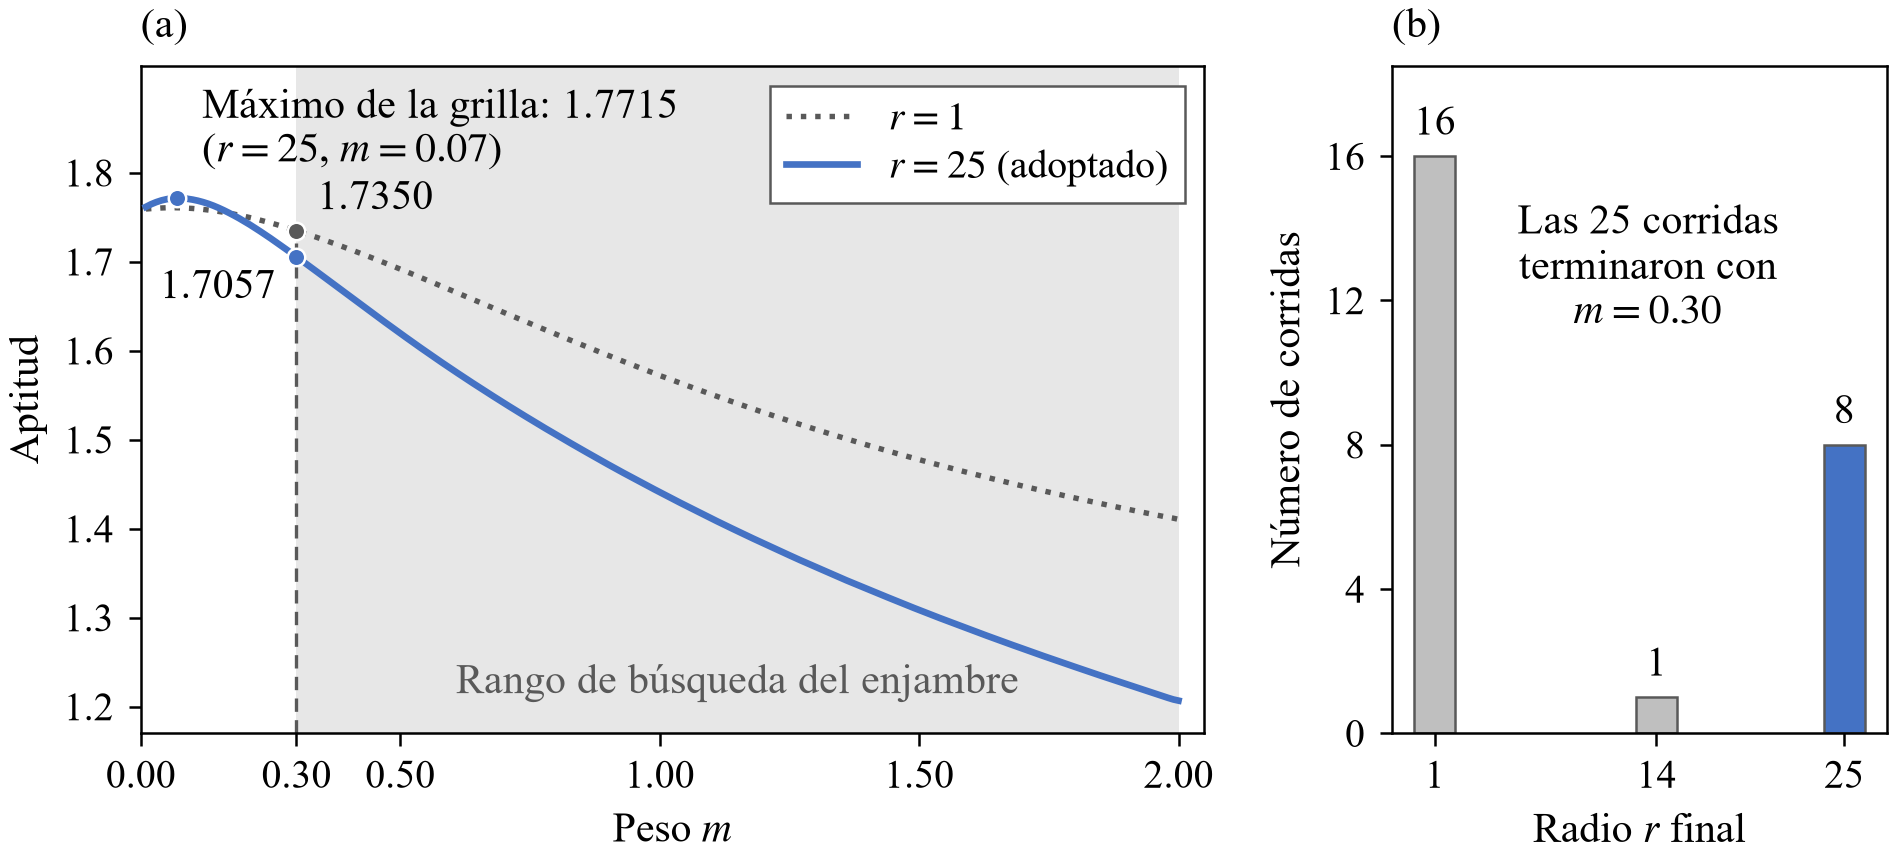
\includegraphics[width=\textwidth]{figuras/fig_ajuste_pso}
\nota{Elaboración propia. (a) Aptitud de la propuesta (Ecuación~\ref{eq:aptitud}) sobre las tres
escenas del ajuste, en función del peso $m$, con los radios $r = 1$ (gris, línea punteada) y $r = 25$
(azul, línea continua). Las
curvas se trazaron con los valores de la grilla, que recorre los pesos de 0.01 a 2.00 cada 0.01. La zona sombreada es
el rango de búsqueda del enjambre, de 0.30 a 2.00, y la línea discontinua marca $m = 0.30$. Los rótulos
indican la aptitud de cada radio en ese peso y el máximo de la grilla. (b) Número de corridas del enjambre
que terminaron en cada radio, de un total de veinticinco, una por configuración de partículas e
iteraciones. En azul está el radio adoptado.}
\end{figure}

Las quinientas corridas de control, que repitieron cada configuración para medir la variación al azar,
mostraron el mismo patrón. En 499 de ellas, el 99.8~\%, el peso terminó en 0.30, y en la restante, en
0.36. El radio volvió a dividirse entre los dos extremos del rango: el
51.4~\% de las corridas terminó en $r = 25$, el 45.6~\% en $r = 1$ y el 3.0~\% restante en otros
radios.

La grilla de cinco mil combinaciones de radio y peso, de la que sale el panel (a), muestra la forma de
la aptitud. Su máximo, 1.7715, se dio en $r = 25$ y $m = 0.07$, fuera del rango de búsqueda.
En cada radio, el mejor peso estuvo entre 0.05 y 0.07, y en los veinticinco radios la aptitud bajó en
cada paso del peso a partir de $m = 0.30$. Dentro del rango de búsqueda, la mayor aptitud fue la de
$r = 1$ y $m = 0.30$, el punto al que llegaron dieciséis corridas. Con el peso en 0.30, la aptitud presentó dos
máximos locales en el radio: uno en $r = 1$, el mayor, y otro en $r = 25$.

Como las corridas se repartieron entre $r = 1$ y $r = 25$, los dos radios se compararon sobre los veinte
pares del corpus, con $m = 0.30$ y las nueve métricas iniciales. El radio 25 fue mejor en las de
actividad, que miden información, contraste y nitidez, y peor en las de fidelidad, que miden el parecido
con las fuentes. Las cinco de actividad son la entropía, la desviación estándar, la eficiencia de
fusión, el gradiente medio y la frecuencia espacial. En cada una, el radio mayor superó a $r = 1$ en los
veinte pares. Las cuatro de fidelidad son la información mutua con cada fuente, la similitud estructural y la
relación señal-ruido de pico. En cada una de estas, $r = 1$ quedó por delante en diecinueve o en veinte
pares.

Con las seis métricas del trabajo, el patrón fue el mismo: $r = 25$ obtuvo valores mayores en las tres
de actividad y menores en las tres de fidelidad. Al pasar de $r = 1$ a $r = 25$, la desviación estándar media subió
de 0.1092 a 0.1439 y el gradiente medio, de 0.0234 a 0.0355. En sentido contrario, la similitud
estructural bajó de 0.7484 a 0.6584 y la información mutua, de 0.9670 a 0.7486. Se adoptó
$r = 25$, uno de los dos resultados del enjambre, porque prioriza el realce. La configuración de la
propuesta que se evalúa en el resto del capítulo es, entonces, $r = 25$ y $m = 0.30$.

El barrido del peso sobre las tres escenas del ajuste mostró que, al aumentar $m$, las métricas de
actividad subieron y las de fidelidad bajaron, con una sola excepción en la propuesta. Con la propuesta
en $r = 25$, la desviación estándar y el gradiente medio subieron en cada paso, desde $m = 0.05$ hasta
$m = 2.0$. La información mutua, la similitud estructural y la relación señal-ruido de pico, en cambio,
bajaron en cada paso. La excepción fue la entropía, que subió hasta $m = 1.2$ y luego descendió. En el
Top-Hat clásico, tanto con $r = 5$ como con $r = 25$, no hubo excepciones: las tres métricas de
actividad subieron y las tres de fidelidad bajaron en cada paso.

\section{Comparación cualitativa}
\label{sec:cualitativa}

Las Figuras~\ref{fig:montaje_kaptein} y~\ref{fig:montaje_humo} presentan dos escenas del corpus, cada
una con sus dos fuentes y las imágenes de los siete métodos. Muestran dos maneras en que las cámaras se
complementan. En la primera, la cámara visible casi no capta a una persona. En la segunda, una
cortina de humo oculta la escena a la cámara visible, y solo la térmica la atraviesa. La comparación es
ilustrativa y no sostiene conclusiones por sí misma.

\begin{figure}[htbp]
\centering
\caption{Fuentes y fusiones de una escena nocturna del TNO (Kaptein 1123)}
\label{fig:montaje_kaptein}
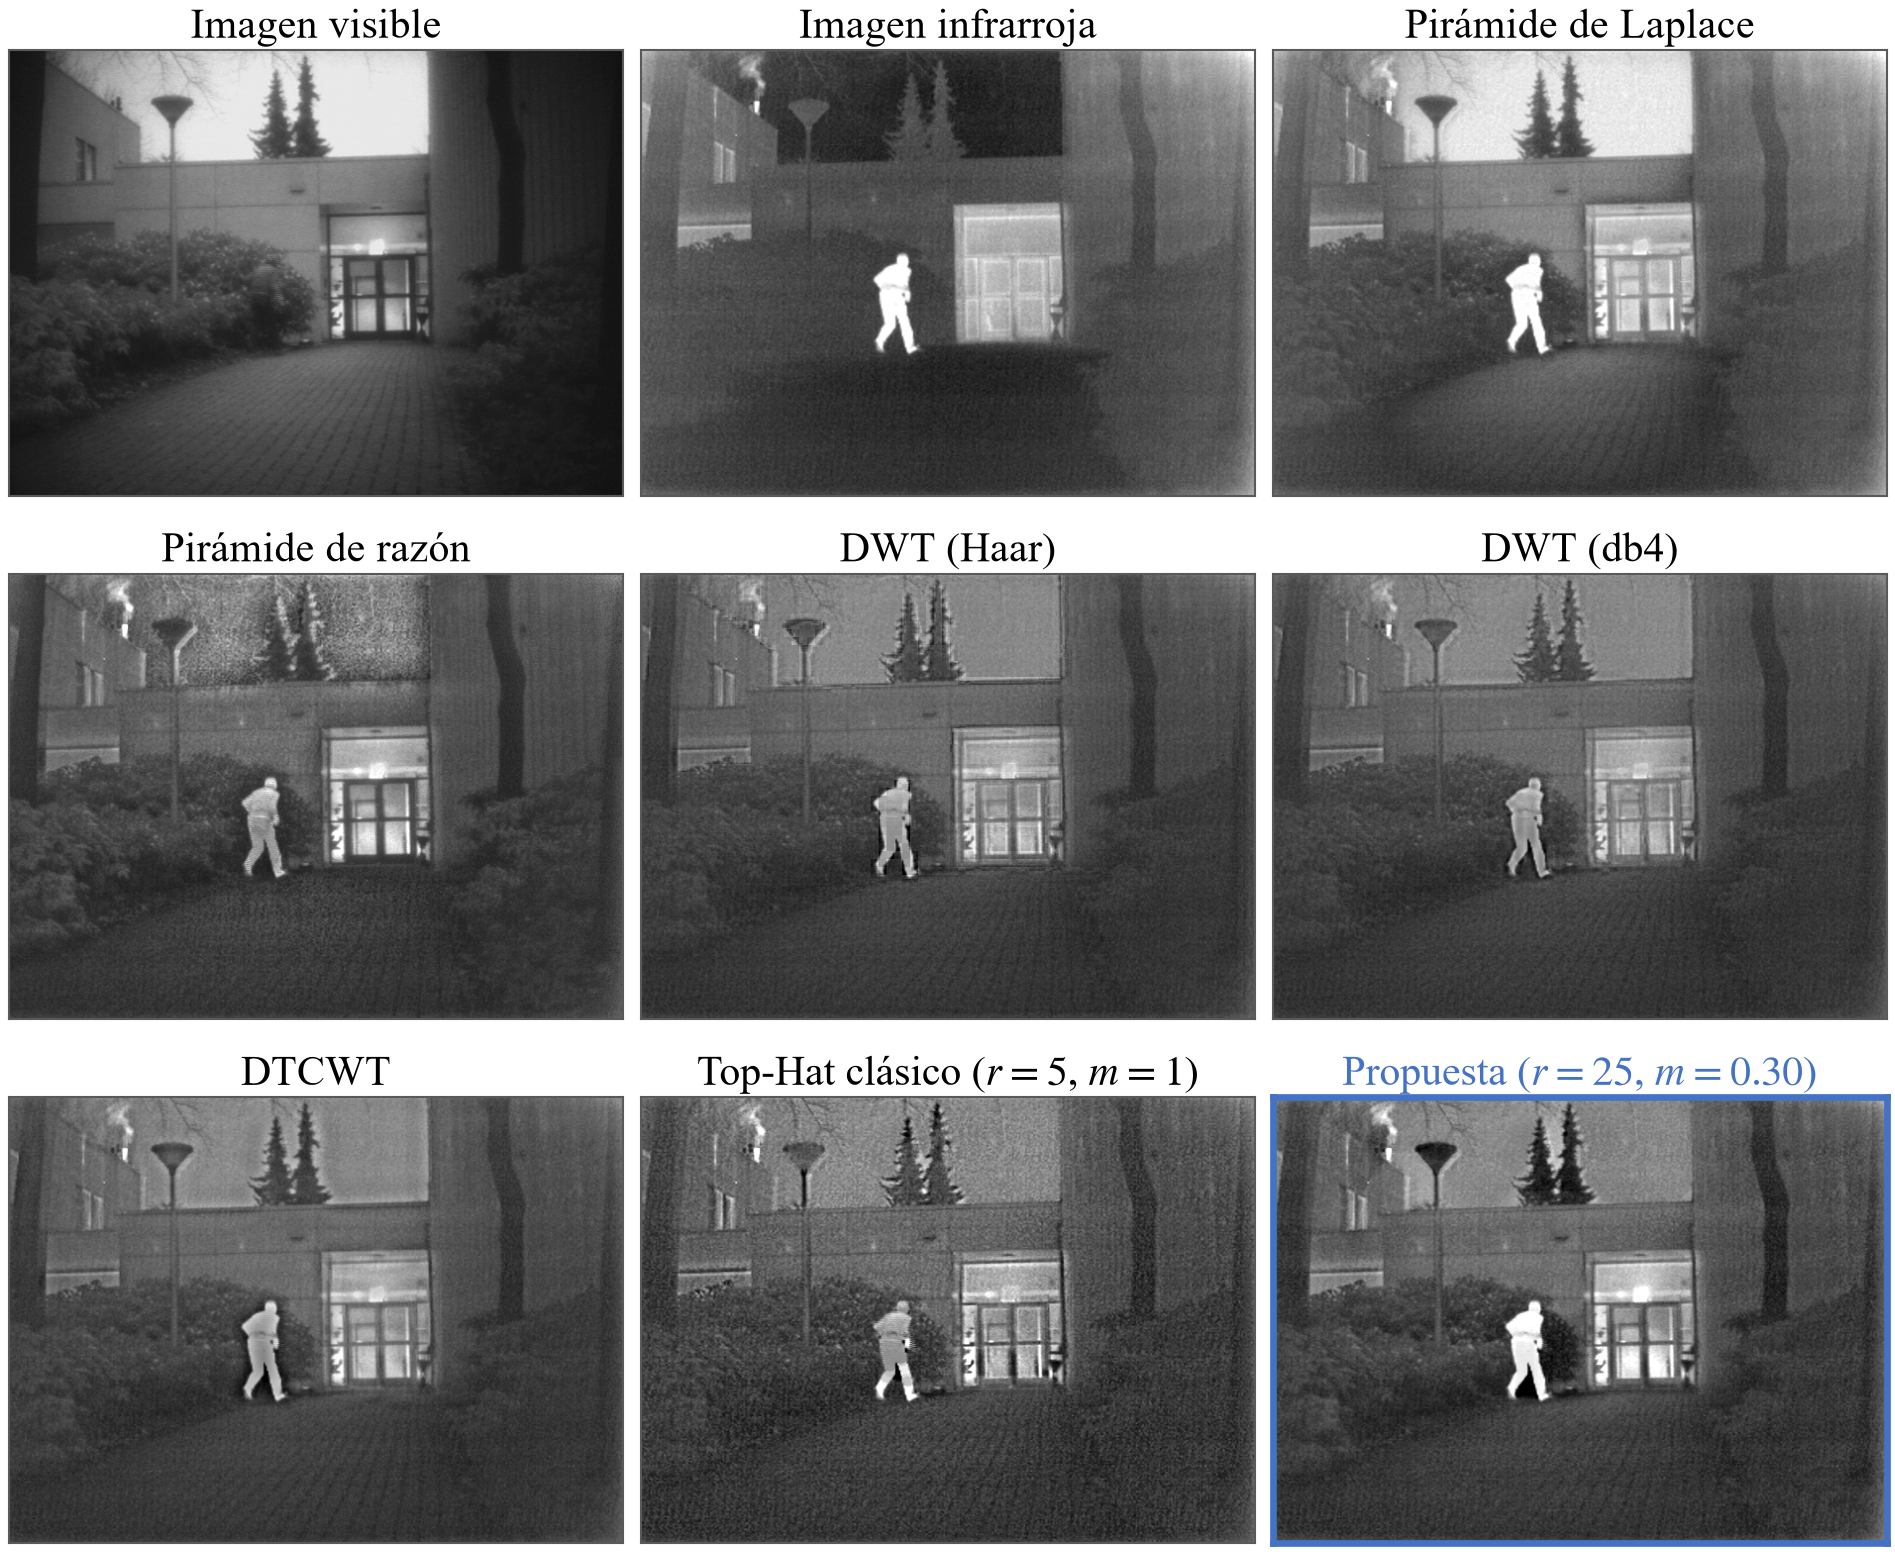
\includegraphics[width=\textwidth]{figuras/montaje_kaptein}
\nota{Elaboración propia a partir de imágenes del \textit{TNO Image Fusion Dataset} \parencite{toet2014, toet2017}. En
la escena hay una persona que en la imagen visible casi no se distingue del fondo. Las dos primeras
imágenes son las fuentes, y las siete siguientes, en orden de lectura, las fusiones de cada método. La
fusión de la propuesta está recuadrada en azul.}
\end{figure}

En la escena nocturna, la imagen visible deja ver con nitidez el edificio, el farol, los árboles y el
sendero de adoquines. La persona que avanza por el sendero, en cambio, se confunde con los arbustos
oscuros. En la infrarroja aparece como una figura brillante, pero el follaje pierde buena parte de su
textura. Las siete fusiones reunieron la silueta de la persona con el fondo de la visible. La pirámide
de razón dejó granulado el cielo, y el Top-Hat clásico, la imagen entera. La pirámide de Laplace y la
propuesta fueron las que más separaron a la persona del fondo. En la propuesta se formó, además, un
borde oscuro alrededor de la figura, con un relleno negro entre las piernas.

\begin{figure}[htbp]
\centering
\caption{Fuentes y fusiones de una escena del TNO con un soldado tendido tras una cortina de humo}
\label{fig:montaje_humo}
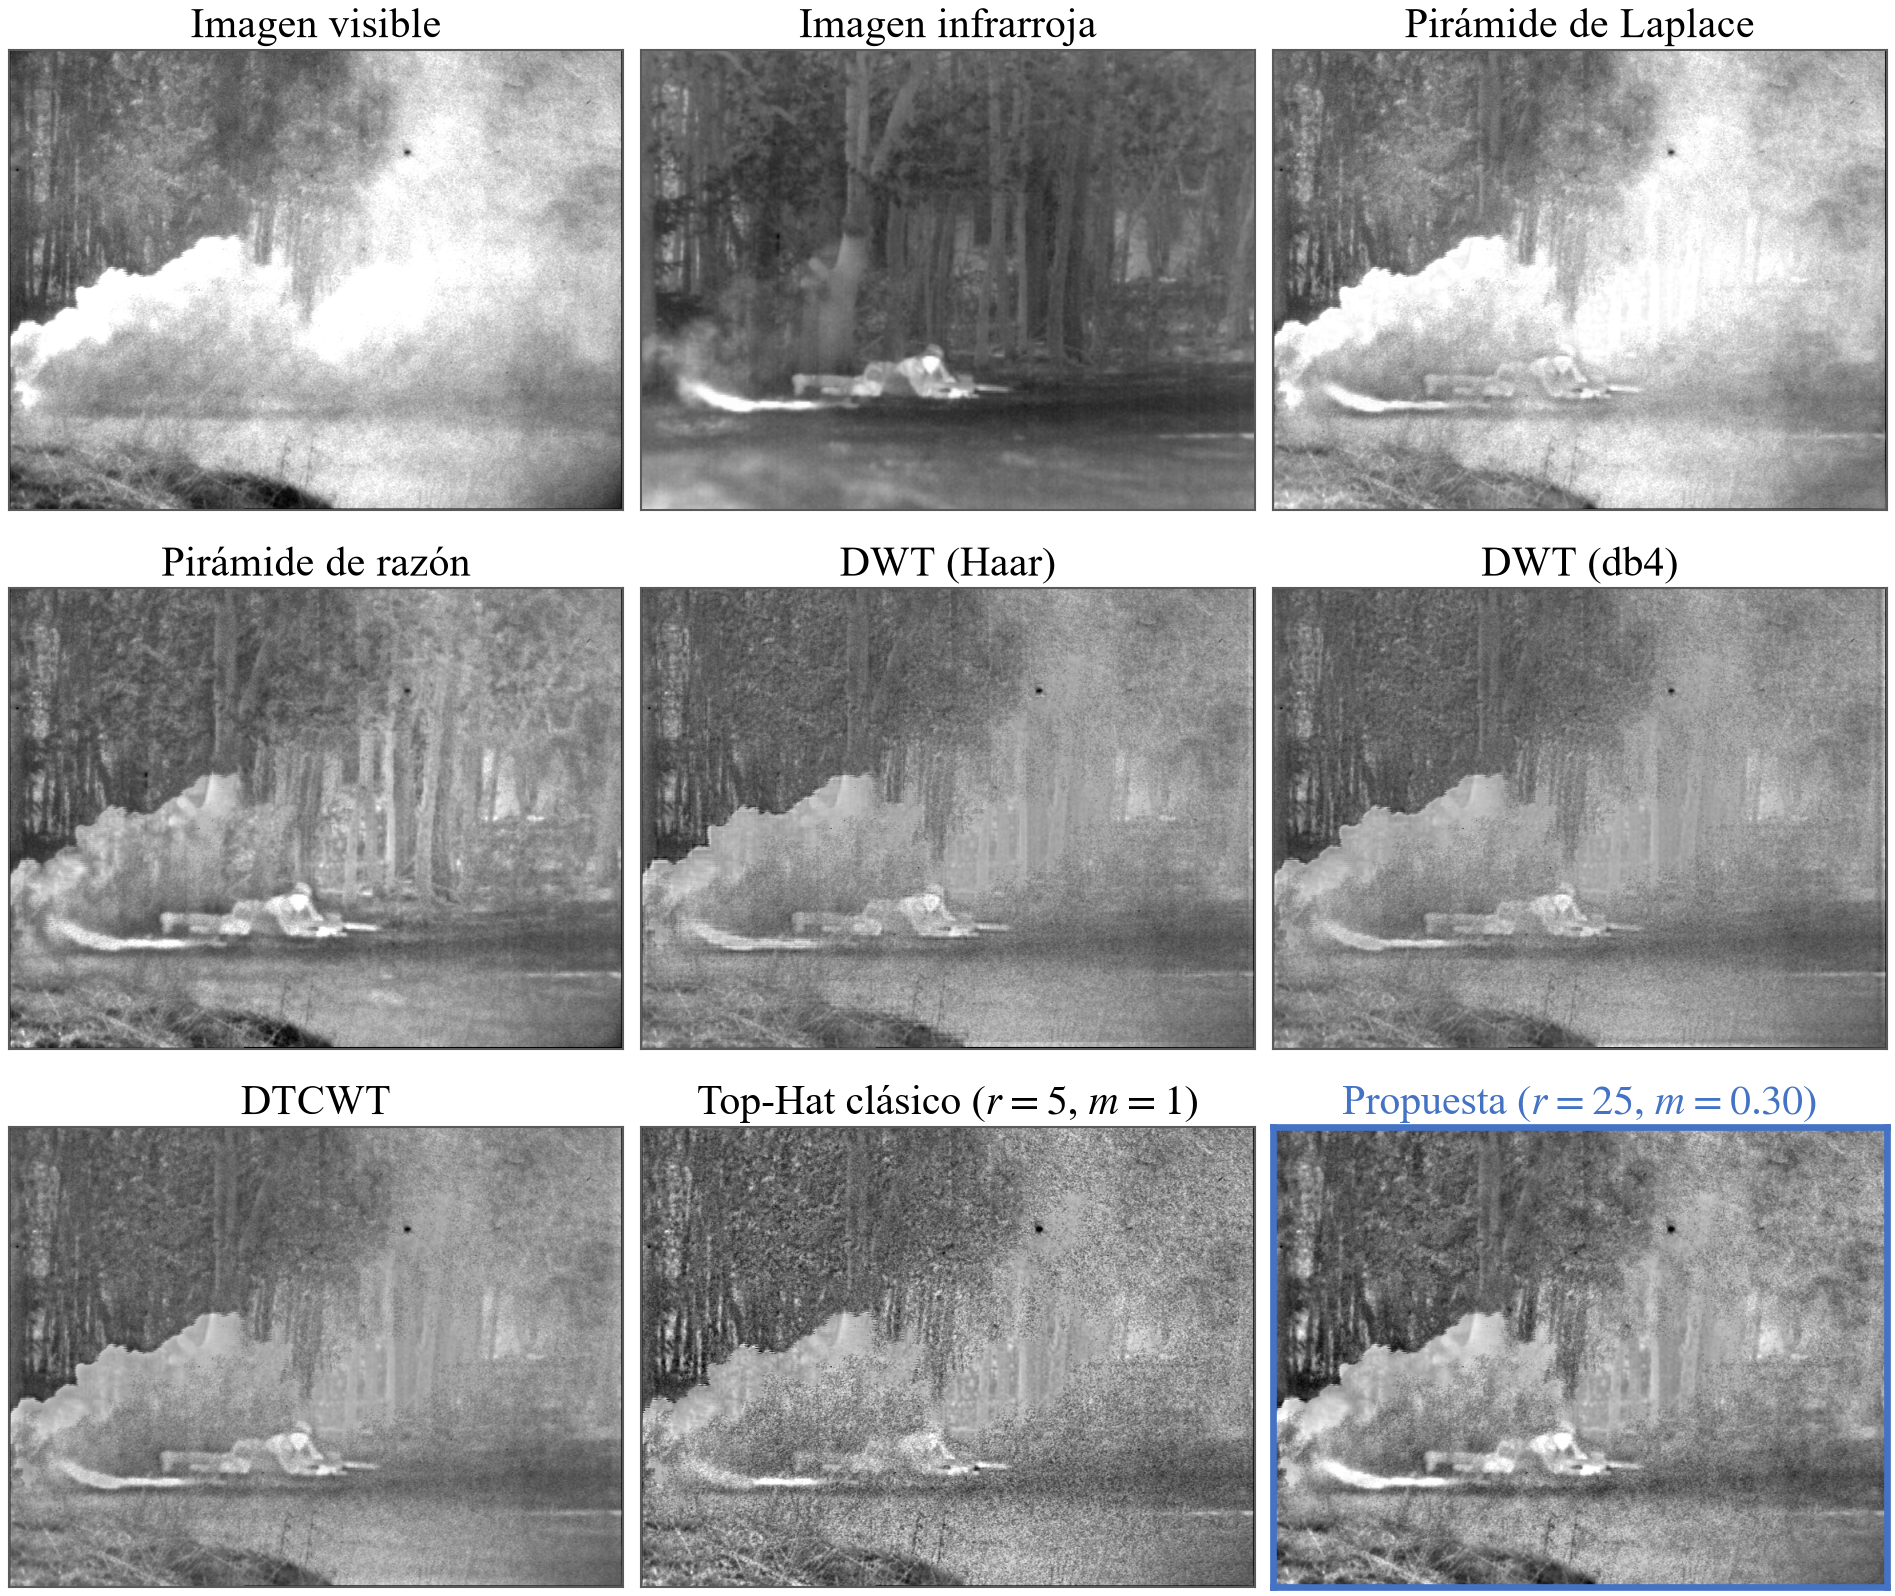
\includegraphics[width=\textwidth]{figuras/montaje_humo}
\nota{Elaboración propia a partir de imágenes del \textit{TNO Image Fusion Dataset} \parencite{toet2014, toet2017}. Es
una de las tres escenas usadas en el ajuste de los parámetros (Sección~\ref{sec:ajuste}). Las dos
primeras imágenes son las fuentes, y las siete siguientes, en orden de lectura, las fusiones de cada
método. La fusión de la propuesta está recuadrada en azul.}
\end{figure}

En la escena del humo, una nube blanca cubre buena parte de la imagen visible y oculta al soldado
tendido detrás de ella. La térmica atraviesa el humo y muestra al soldado junto con los troncos del
bosque. La pirámide de Laplace conservó gran parte del brillo del humo, y en ella el soldado apenas se
insinúa. Las otras seis fusiones atenuaron la cortina y recuperaron la figura del soldado. El Top-Hat
clásico volvió a ser el más granulado. La propuesta, como él, mostró en los árboles y en el pasto más
textura que los cinco métodos multiescala. También dejó algo de grano, aunque menos que el del
Top-Hat clásico.

\section{Resultados cuantitativos}
\label{sec:cuantitativos}

La Tabla~\ref{tab:medias_seis} reúne la media de cada métrica sobre los veinte pares. En las seis, un
valor mayor es mejor. Las tres primeras métricas de la tabla son las de actividad y las tres últimas,
las de fidelidad.

\begin{table}[htbp]
\centering
\caption{Media de las seis métricas por método, sobre los veinte pares del corpus}
\label{tab:medias_seis}
\begin{tabular}{lcccccc}
\toprule
\textbf{Método} & \textbf{EN} & \textbf{SD} & \textbf{MG} & \textbf{MI} & \textbf{SSIM} & \textbf{PSNR} \\
\midrule
Propuesta & \textbf{6.9855} & 0.1439 & 0.0355 & 0.7486 & 0.6584 & 16.84 \\
DTCWT & 6.6877 & 0.1172 & 0.0255 & 0.8755 & \textbf{0.7249} & 17.60 \\
Pirámide de Laplace & 6.8400 & \textbf{0.1550} & 0.0252 & \textbf{1.4210} & 0.7059 & 14.94 \\
Pirámide de razón & 6.8098 & 0.1271 & 0.0275 & 0.7995 & 0.7051 & 17.37 \\
DWT (db4) & 6.6445 & 0.1132 & 0.0260 & 0.8828 & 0.7162 & \textbf{17.65} \\
Top-Hat clásico & 6.9220 & 0.1352 & \textbf{0.0478} & 0.6398 & 0.5640 & 16.87 \\
DWT (Haar) & 6.6816 & 0.1166 & 0.0275 & 0.8711 & 0.7014 & 17.59 \\
\bottomrule
\end{tabular}
\nota{Elaboración propia. En las seis métricas, un valor mayor es mejor, y la negrita marca el mejor valor de cada columna. Los métodos siguen el orden del rango promedio (Tabla~\ref{tab:ranking_seis}). EN: entropía. SD: desviación estándar. MG: gradiente medio. MI: información mutua. SSIM: similitud estructural. En MI y en SSIM, el valor es el promedio del calculado contra la imagen visible y del calculado contra la infrarroja. PSNR: relación señal-ruido de pico, en decibelios, calculada con el promedio de los dos errores cuadráticos medios. DWT (Haar) y DWT (db4) son la misma transformada con dos bases distintas (Sección~\ref{sec:comparativos}). Propuesta: el algoritmo de fusión presentado en este trabajo.}
\end{table}


En las métricas de actividad, la propuesta quedó siempre primera o segunda. Obtuvo la mayor entropía de
los siete métodos, 6.9855, seguida por el Top-Hat clásico, con 6.9220. En desviación estándar quedó
segunda, con 0.1439, detrás de la pirámide de Laplace, que llegó a 0.1550. También fue segunda en gradiente medio, con 0.0355, esta vez detrás del
Top-Hat clásico, con 0.0478. En entropía y en gradiente medio, los dos métodos morfológicos ocuparon los
dos primeros puestos, por delante de los cinco multiescala.

En fidelidad, el orden cambió: la propuesta quedó sexta de siete en cada métrica. Obtuvo 0.7486
en información mutua, 0.6584 en similitud estructural y 16.84 decibelios en relación señal-ruido de
pico. Cada una de esas métricas tuvo un método distinto en el primer puesto. En información mutua fue
la pirámide de Laplace, con 1.4210; en similitud estructural, la DTCWT, con 0.7249, y en relación
señal-ruido de pico, la DWT (db4), con 17.65 decibelios. Solo un método quedó por debajo de
la propuesta: el Top-Hat clásico en las dos primeras y la pirámide de Laplace en la tercera.

La Figura~\ref{fig:metricas_cajas} muestra los veinte valores de cada método en cada métrica, y no solo
su media. La variación de un par a otro es grande frente a la distancia entre las medias. En relación
señal-ruido de pico, por ejemplo, la propuesta va de 11.12 a 21.65 decibelios según el par, mientras
que las medias de los siete métodos quedan entre 14.94 y 17.65. Por eso las cajas se superponen en buena
parte, aunque algunas se separan del resto. En gradiente medio, las de la propuesta y del Top-Hat clásico
quedan enteras a la derecha de las de los cinco métodos multiescala. En información mutua, la de la
pirámide de Laplace queda a la derecha de todas las demás.

\begin{figure}[htbp]
\centering
\caption{Valores de las seis métricas en los veinte pares, por método}
\label{fig:metricas_cajas}
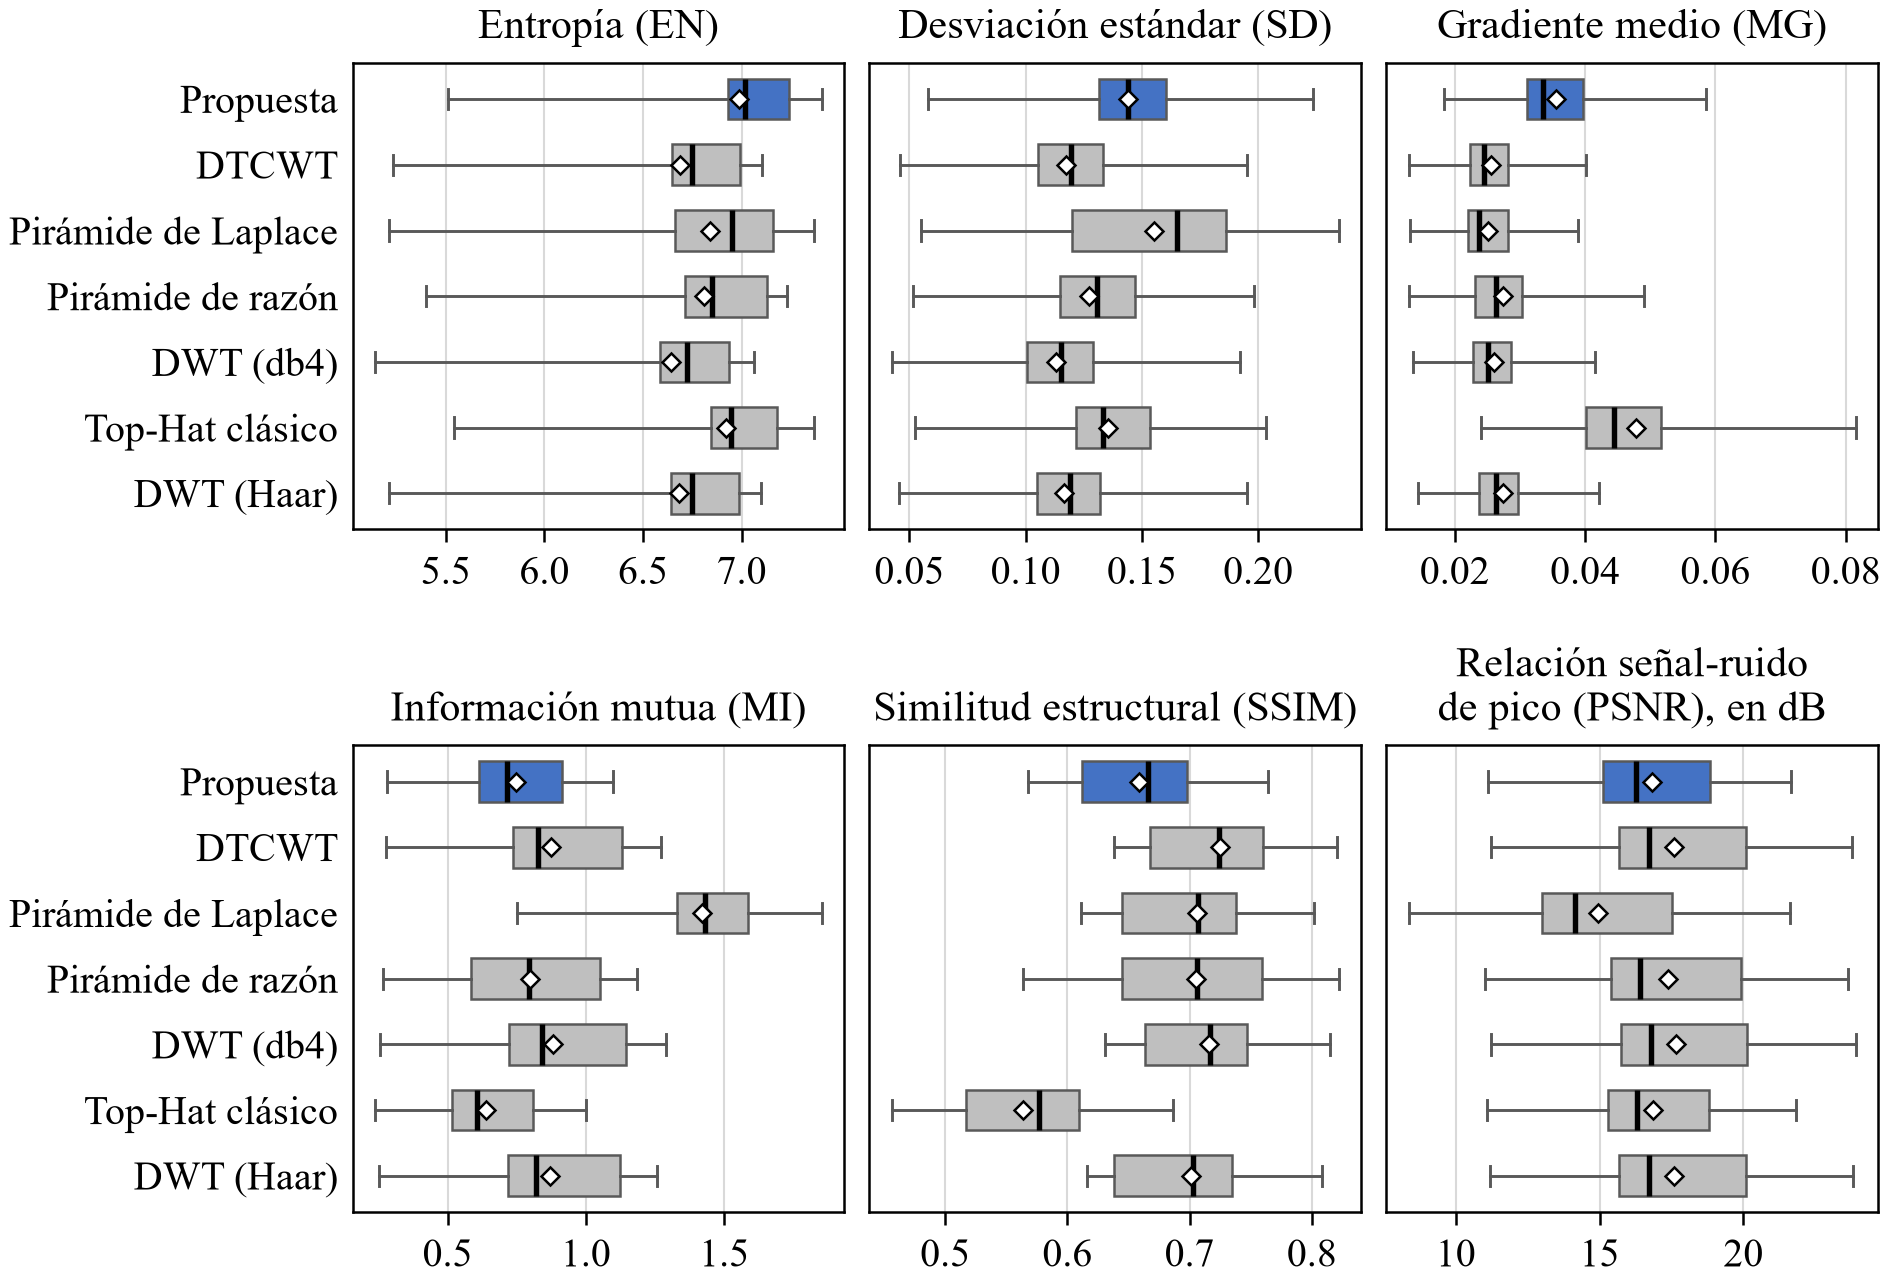
\includegraphics[width=\textwidth]{figuras/fig_metricas_cajas}
\nota{Elaboración propia. Cada caja reúne los veinte valores de un método en una métrica, uno por par
del corpus. La caja abarca la mitad central de esos valores, del primer al tercer cuartil, y la línea
negra es la mediana. El rombo blanco es la media de la Tabla~\ref{tab:medias_seis}, y los bigotes
llegan al mínimo y al máximo. Arriba están las tres métricas de actividad y abajo, las tres de
fidelidad. Los métodos siguen el orden del rango promedio (Tabla~\ref{tab:ranking_seis}), y la propuesta
está en azul.}
\end{figure}

\section{Análisis estadístico}
\label{sec:estadistico}

Ni las medias ni las cajas indican si las diferencias se repiten par a par. Para eso se siguió el
análisis de la Sección~\ref{sec:protocolo-calidad}: la prueba de Friedman por métrica, la clasificación
por rango promedio, los contrastes de Wilcoxon y varias comprobaciones de la solidez del orden.

\subsection{Prueba de Friedman y rango promedio}
\label{sec:res-friedman}

La prueba de Friedman, con los veinte pares como bloques y seis grados de libertad, encontró diferencias
entre los siete métodos en las seis métricas (Tabla~\ref{tab:friedman_seis}). El valor de $p$ fue menor
que 0.001 en todas. El estadístico varió entre 88.3, en entropía, y 111.8, en relación señal-ruido de
pico.

\begin{table}[htbp]
\centering
\caption{Prueba de Friedman por métrica, con siete métodos y veinte pares}
\label{tab:friedman_seis}
\begin{tabular}{lccc}
\toprule
\textbf{Métrica} & \textbf{\boldmath $\chi^2$} & \textbf{\boldmath $p$} & \textbf{¿Difieren?} \\
\midrule
EN & 88.3 & $< 0.001$ & sí \\
SD & 105.1 & $< 0.001$ & sí \\
MG & 101.7 & $< 0.001$ & sí \\
MI & 91.2 & $< 0.001$ & sí \\
SSIM & 100.5 & $< 0.001$ & sí \\
PSNR & 111.8 & $< 0.001$ & sí \\
\bottomrule
\end{tabular}
\nota{Elaboración propia. La prueba contrasta si los rangos promedio de los métodos difieren más de lo esperable por azar. Con siete métodos, tiene seis grados de libertad. La columna ¿Difieren? indica si la diferencia fue significativa, como ocurrió en las seis métricas. En ese caso, algunos métodos quedan mejor o peor ubicados de forma sistemática, par tras par.}
\end{table}


La Tabla~\ref{tab:ranking_seis} y la Figura~\ref{fig:ranking_seis} muestran el rango promedio de cada
método. Es el puesto medio que ocupa sobre los pares y las métricas, de modo que un valor menor es
mejor. La propuesta encabezó la clasificación con 3.642, seguida por la DTCWT, con 3.783, y por la
pirámide de Laplace, con 3.908. Su ventaja sobre la DTCWT fue de 0.14 puestos y no se sometió a una prueba propia. El Top-Hat
clásico quedó sexto de siete, con 4.242.

\begin{table}[htbp]
\centering
\caption{Rango promedio de cada método, por métrica y global}
\label{tab:ranking_seis}
\begin{tabular}{clccccccc}
\toprule
\textbf{Puesto} & \textbf{Método} & \textbf{EN} & \textbf{SD} & \textbf{MG} & \textbf{MI} & \textbf{SSIM} & \textbf{PSNR} & \textbf{Global} \\
\midrule
1 & Propuesta & 1.50 & 1.65 & 2.00 & 5.45 & 5.90 & 5.35 & \textbf{3.642} \\
2 & DTCWT & 4.90 & 5.05 & 6.05 & 3.15 & 1.30 & 2.25 & 3.783 \\
3 & Pirámide de Laplace & 3.25 & 2.00 & 6.25 & 1.20 & 3.80 & 6.95 & 3.908 \\
4 & Pirámide de razón & 3.55 & 3.60 & 4.65 & 4.95 & 3.00 & 4.35 & 4.017 \\
5 & DWT (db4) & 6.85 & 7.00 & 4.75 & 2.65 & 2.50 & 1.00 & 4.125 \\
6 & Top-Hat clásico & 2.45 & 2.85 & 1.00 & 6.80 & 7.00 & 5.35 & 4.242 \\
7 & DWT (Haar) & 5.50 & 5.85 & 3.30 & 3.80 & 4.50 & 2.75 & 4.283 \\
\bottomrule
\end{tabular}
\nota{Elaboración propia. En cada par y en cada métrica, el rango 1 corresponde al mejor método. Cada columna de métrica promedia esos rangos sobre los pares, y la columna Global promedia las seis columnas de métrica. Un valor menor es mejor, y la negrita marca el mejor rango global. La prueba de Friedman opera sobre estos mismos rangos. Propuesta: el algoritmo de fusión presentado en este trabajo.}
\end{table}


\begin{figure}[htbp]
\centering
\caption{Rango promedio de cada método sobre las seis métricas}
\label{fig:ranking_seis}
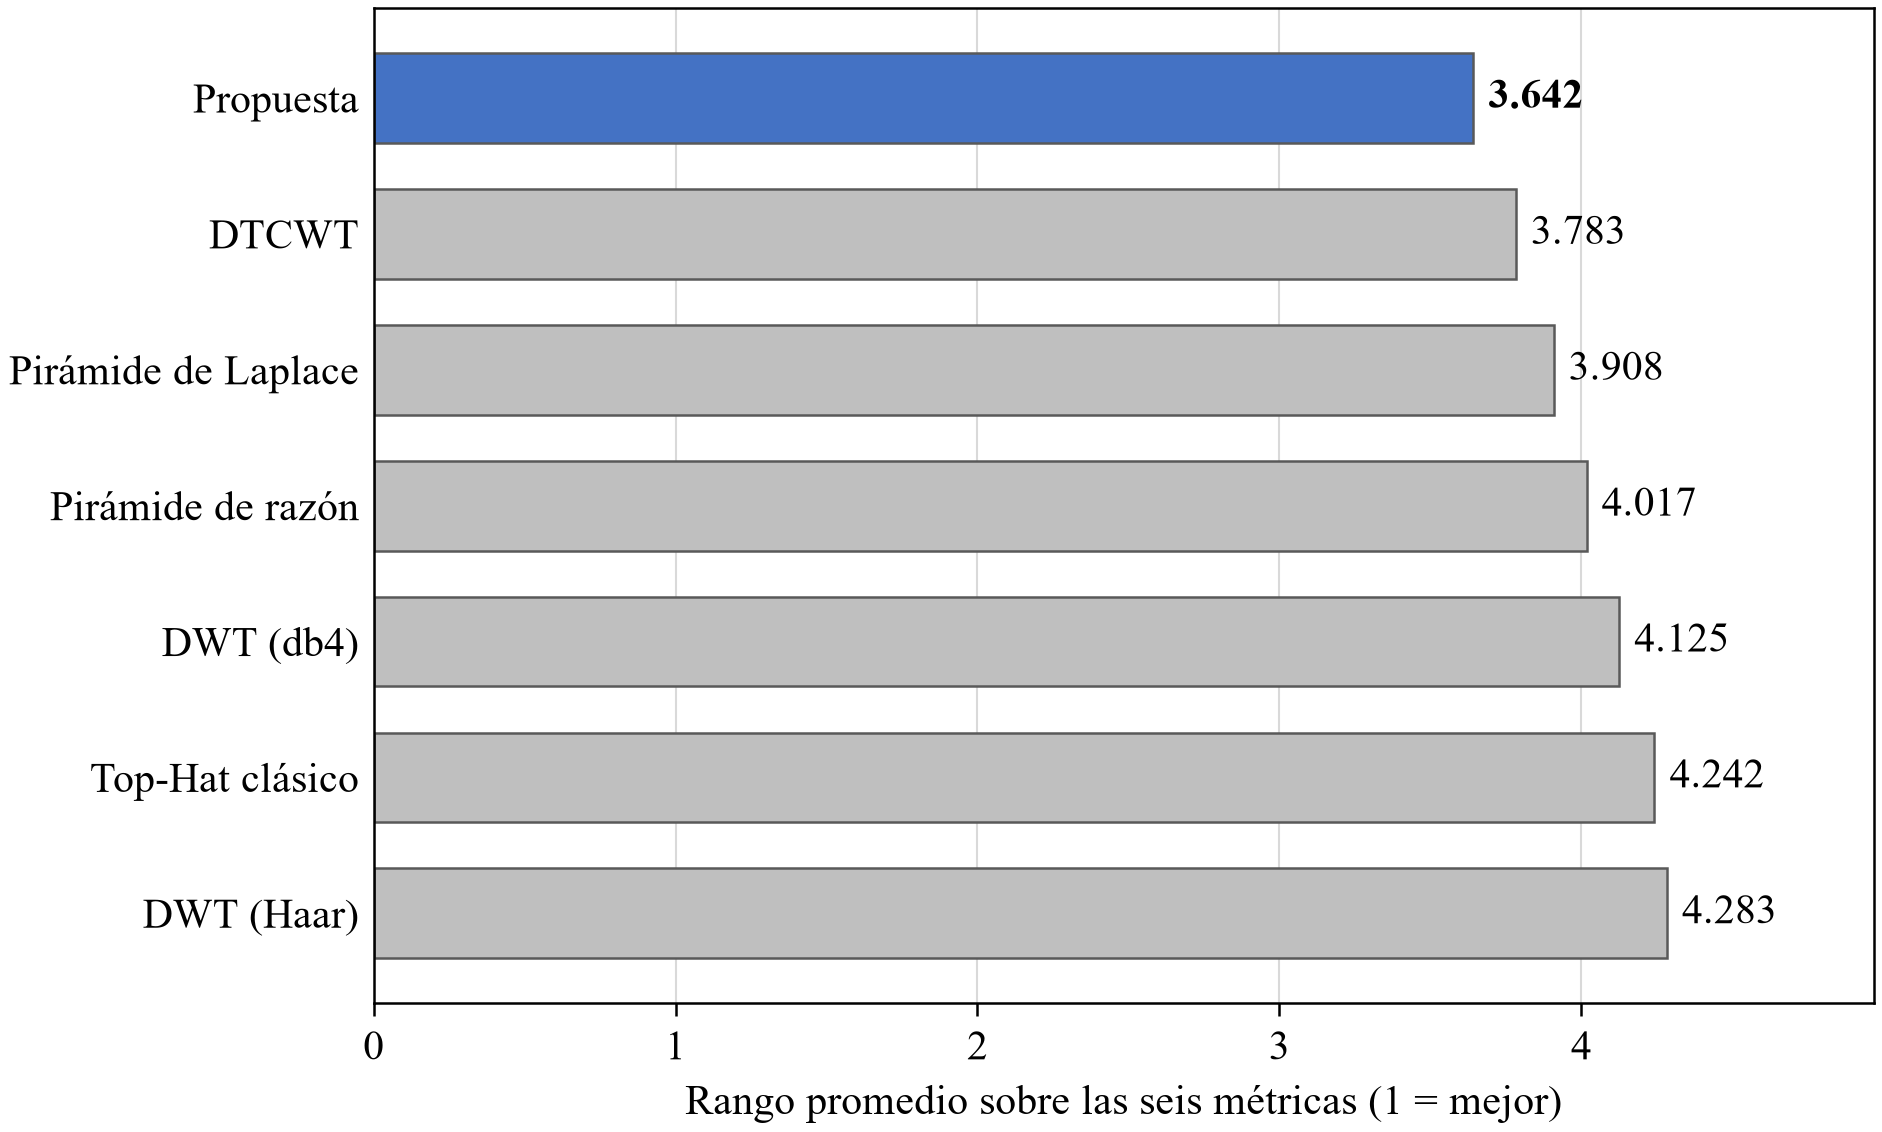
\includegraphics[width=\textwidth]{figuras/fig_ranking_seis}
\nota{Elaboración propia. Cada barra es el puesto medio del método sobre los pares y las métricas, y un
valor menor indica un método mejor ubicado. La propuesta está en azul.}
\end{figure}

Calculado por separado en cada grupo de métricas, el rango promedio muestra perfiles distintos. En las
tres de actividad, la propuesta tuvo 1.717, el mejor de los siete, y en las tres de fidelidad, 5.567, el sexto.
La DTCWT tuvo el perfil opuesto: 5.333 en actividad, sexta, y 2.233 en fidelidad, segunda. La suma de
los dos rangos fue de 7.28 en la propuesta y de 7.57 en la DTCWT. El Top-Hat clásico, sexto en la
clasificación global, obtuvo 2.100 en actividad y 6.383 en fidelidad.

\subsection{Contrastes de Wilcoxon}
\label{sec:res-wilcoxon}

Como la prueba de Friedman resultó significativa en las seis métricas, en cada una se aplicaron los
once contrastes de Wilcoxon, que comparan dos métodos sobre los mismos pares de imágenes. Son sesenta y
seis en total, y sus valores de $p$ se corrigieron con el procedimiento de Holm dentro de cada métrica. La
Tabla~\ref{tab:wilcoxon_resumen} resume los que comparan a la propuesta con los demás métodos. Los once
de cada métrica, incluidos los del Top-Hat clásico frente a los cinco multiescala, figuran en los Anexos
(Tabla~\ref{tab:wilcoxon_completa}).

\begin{table}[htbp]
\centering
\caption{Contrastes de Wilcoxon pareados de la propuesta frente a los demás métodos}
\label{tab:wilcoxon_resumen}
\setlength{\tabcolsep}{5pt}
\begin{tabular}{lccclcc}
\toprule
& \multicolumn{3}{c}{\textbf{Contra los cinco multiescala}} & \multicolumn{3}{c}{\textbf{Contra el Top-Hat clásico}} \\
\cmidrule(lr){2-4}\cmidrule(lr){5-7}
\textbf{Métrica} & \textbf{Gana} & \textbf{Pierde} & \textbf{Empata} & \textbf{Resultado} & \textbf{Diferencia} & \textbf{\boldmath $p$ corregido} \\
\midrule
EN & 5 & 0 & 0 & gana & 0.0636 & $< 0.001$ \\
SD & 4 & 0 & 1 & gana & 0.0087 & $< 0.001$ \\
MG & 5 & 0 & 0 & pierde & $-$0.0123 & $< 0.001$ \\
MI & 0 & 4 & 1 & gana & 0.1089 & $< 0.001$ \\
SSIM & 0 & 5 & 0 & gana & 0.0944 & $< 0.001$ \\
PSNR & 1 & 4 & 0 & empata & $-$0.0319 & 0.674 \\
\bottomrule
\end{tabular}
\nota{Elaboración propia. Gana, Pierde y Empata cuentan los contrastes de la propuesta con los cinco métodos multiescala. Resultado, Diferencia y $p$ corregido se refieren a su contraste con el Top-Hat clásico. Un contraste significativo al 5~\% después de corregir por comparaciones múltiples, con Holm sobre los once contrastes de cada métrica, cuenta como victoria o derrota de la propuesta según el signo de la diferencia de medias. Uno no significativo cuenta como empate. Diferencia: media de la propuesta menos media del Top-Hat clásico, en las unidades de cada métrica (decibelios en PSNR). El Top-Hat clásico se usó con radio 5 y peso 1.}
\end{table}


Frente a los cinco métodos multiescala, la propuesta ganó casi todos los contrastes de actividad y
perdió casi todos los de fidelidad. Ganó los cinco de entropía y los cinco de gradiente medio, y en
desviación estándar ganó cuatro y empató con la pirámide de Laplace. En fidelidad perdió los cinco
contrastes de similitud estructural. En información mutua perdió cuatro y empató con la pirámide de
razón, y en relación señal-ruido de pico perdió cuatro y le ganó a la pirámide de Laplace.

Frente al Top-Hat clásico, la propuesta ganó en cuatro métricas, perdió en una y empató en otra. Las
cuatro victorias tuvieron un $p$ corregido menor que 0.001, con diferencias de medias de 0.0636 en
entropía, 0.0087 en desviación estándar, 0.1089 en información mutua y 0.0944 en similitud
estructural. La derrota fue en gradiente medio, con una diferencia de $-0.0123$ y un $p$ corregido también menor que 0.001. En relación señal-ruido de pico, la
diferencia de $-0.0319$ decibelios no fue significativa: su $p$ corregido fue de 0.674, de modo que esa
métrica cuenta como empate.

\subsection{Solidez del orden}
\label{sec:res-robustez}

Al repetir el análisis con trece bloques, uno por escena, la cabeza de la clasificación no cambió: la
propuesta siguió primera, con 3.590, y la DTCWT, segunda, con 3.756. La prueba de Friedman volvió a
ser significativa en las seis métricas, con $p$ menor que 0.001 y estadísticos entre 56.6 y 73.0. Los sesenta y seis contrastes de
Wilcoxon conservaron su signo, y sesenta y cinco conservaron además su decisión. El único que cambió fue
el del Top-Hat clásico frente a la pirámide de razón en desviación estándar. Su $p$ corregido pasó de
0.005 con veinte pares a 0.098 con trece bloques, y el contraste dejó de ser significativo.

El puesto de la propuesta, en cambio, dependió del conjunto de métricas. Con las nueve métricas
iniciales quedó primera, con 3.394, seguida por la pirámide de Laplace, con 3.911. Con las diecisiete
que se calcularon quedó tercera, con 3.459, detrás de la pirámide de Laplace, con 3.147, y de la DTCWT,
con 3.259. Las ocho métricas que se suman a las nueve iniciales, entre ellas Qabf, Nabf, SCD, VIF y
FMI, comparan la fusión con sus fuentes, de modo que doce de las diecisiete son de ese tipo. Las tres
clasificaciones usan la misma escala, de 1 a 7, pero promedian métricas distintas; por eso se compara
el puesto y no el valor.

En el control con imágenes degradadas, que mide si el ruido recibe premio, se ordenaron catorce entradas
con las seis métricas, en una escala de 1 a 14. Las entradas fueron los siete métodos, el promedio simple y seis
imágenes degradadas a partir de ese promedio. El promedio con ruido ganó puestos a medida que crecía el
ruido. Con una desviación estándar del ruido de 0.02 quedó decimotercero; con 0.05, duodécimo, y con
0.10, décimo. Con 0.20 empató en el octavo puesto con el Top-Hat clásico, ambos con 7.483, y fue la mejor de las catorce entradas en las tres métricas de
actividad. El Top-Hat clásico quedó así como el último de los siete métodos en ese control.

La cabeza del control la ocuparon la pirámide de Laplace, con 6.633, y el promedio simple, con 6.650.
La propuesta quedó tercera, con 6.725. Ese puesto depende de las entradas que se ordenan. Con
solo los siete métodos y el promedio simple, en una escala de 1 a 8, la propuesta queda primera, con
4.142, y el promedio, sexto, con 4.633. El cambio lo producen las dos versiones desenfocadas, que en
puesto medio quedan delante de la propuesta en las tres métricas de fidelidad y detrás del promedio
simple en las seis.

\section{Aplicación a la detección de objetos}
\label{sec:deteccion}

Los treinta detectores previstos, tres por cada una de las diez entradas, completaron su entrenamiento.
Esta sección presenta primero los objetos de una sola cámara y las tasas de acierto de cada entrada.
Después compara la propuesta con el Top-Hat clásico, y al final reúne las medidas secundarias y el
seguimiento del entrenamiento.

\subsection{Objetos de una sola cámara y tasas de acierto}
\label{sec:res-tasas}

Los cuadros de seguimiento sirvieron para calibrar el umbral principal. En ellos, con el umbral de 0.25,
los detectores de la visible cometieron en promedio 0.948 falsos positivos de personas y luces por
imagen. Los umbrales con que cada detector más se acercó a ese valor, que forman el umbral principal de la
Sección~\ref{sec:det-medida}, quedaron entre 0.24 y 0.27.

Con el umbral principal, los detectores de la visible y de la infrarroja definieron 211 objetos vistos
solo por la visible y 622 vistos solo por la infrarroja. Otros 724 los encontraron los detectores de
las dos cámaras. Con el umbral fijo de 0.25, esos tres conjuntos tuvieron 209, 624 y 728 objetos, y con
el de mejor equilibrio por clase, 197, 633 y 667. Los objetos de una sola cámara quedaron repartidos en
diez de los once grupos de la prueba. El reparto fue muy desigual: de los 211 objetos de solo la
visible, 176 provienen de dos grupos, con 86 y 90. El de 90, el mayor de la prueba, reúne también 219
de los 622 de solo la infrarroja.

La Figura~\ref{fig:m3fd_ejemplo} muestra un cuadro nocturno de la prueba con dos objetos de una sola
cámara, uno de cada cámara. El semáforo encendido, que M3FD marca como luz, solo lo encuentran los
detectores de la imagen visible, y la persona del borde izquierdo, solo los de la infrarroja. Con la
primera semilla, es decir, en el primer entrenamiento de cada entrada, el detector del Top-Hat clásico
encontró el semáforo y el de la propuesta no. Ninguno de los dos encontró a la persona del borde, y
los dos encontraron a la que está delante del auto y a otra lejana. Como se trata de un solo
cuadro y una sola semilla, el ejemplo no representa el resultado de conjunto.

\begin{figure}[htbp]
\centering
\caption{Detecciones del Top-Hat clásico y de la propuesta en un cuadro nocturno de M3FD}
\label{fig:m3fd_ejemplo}
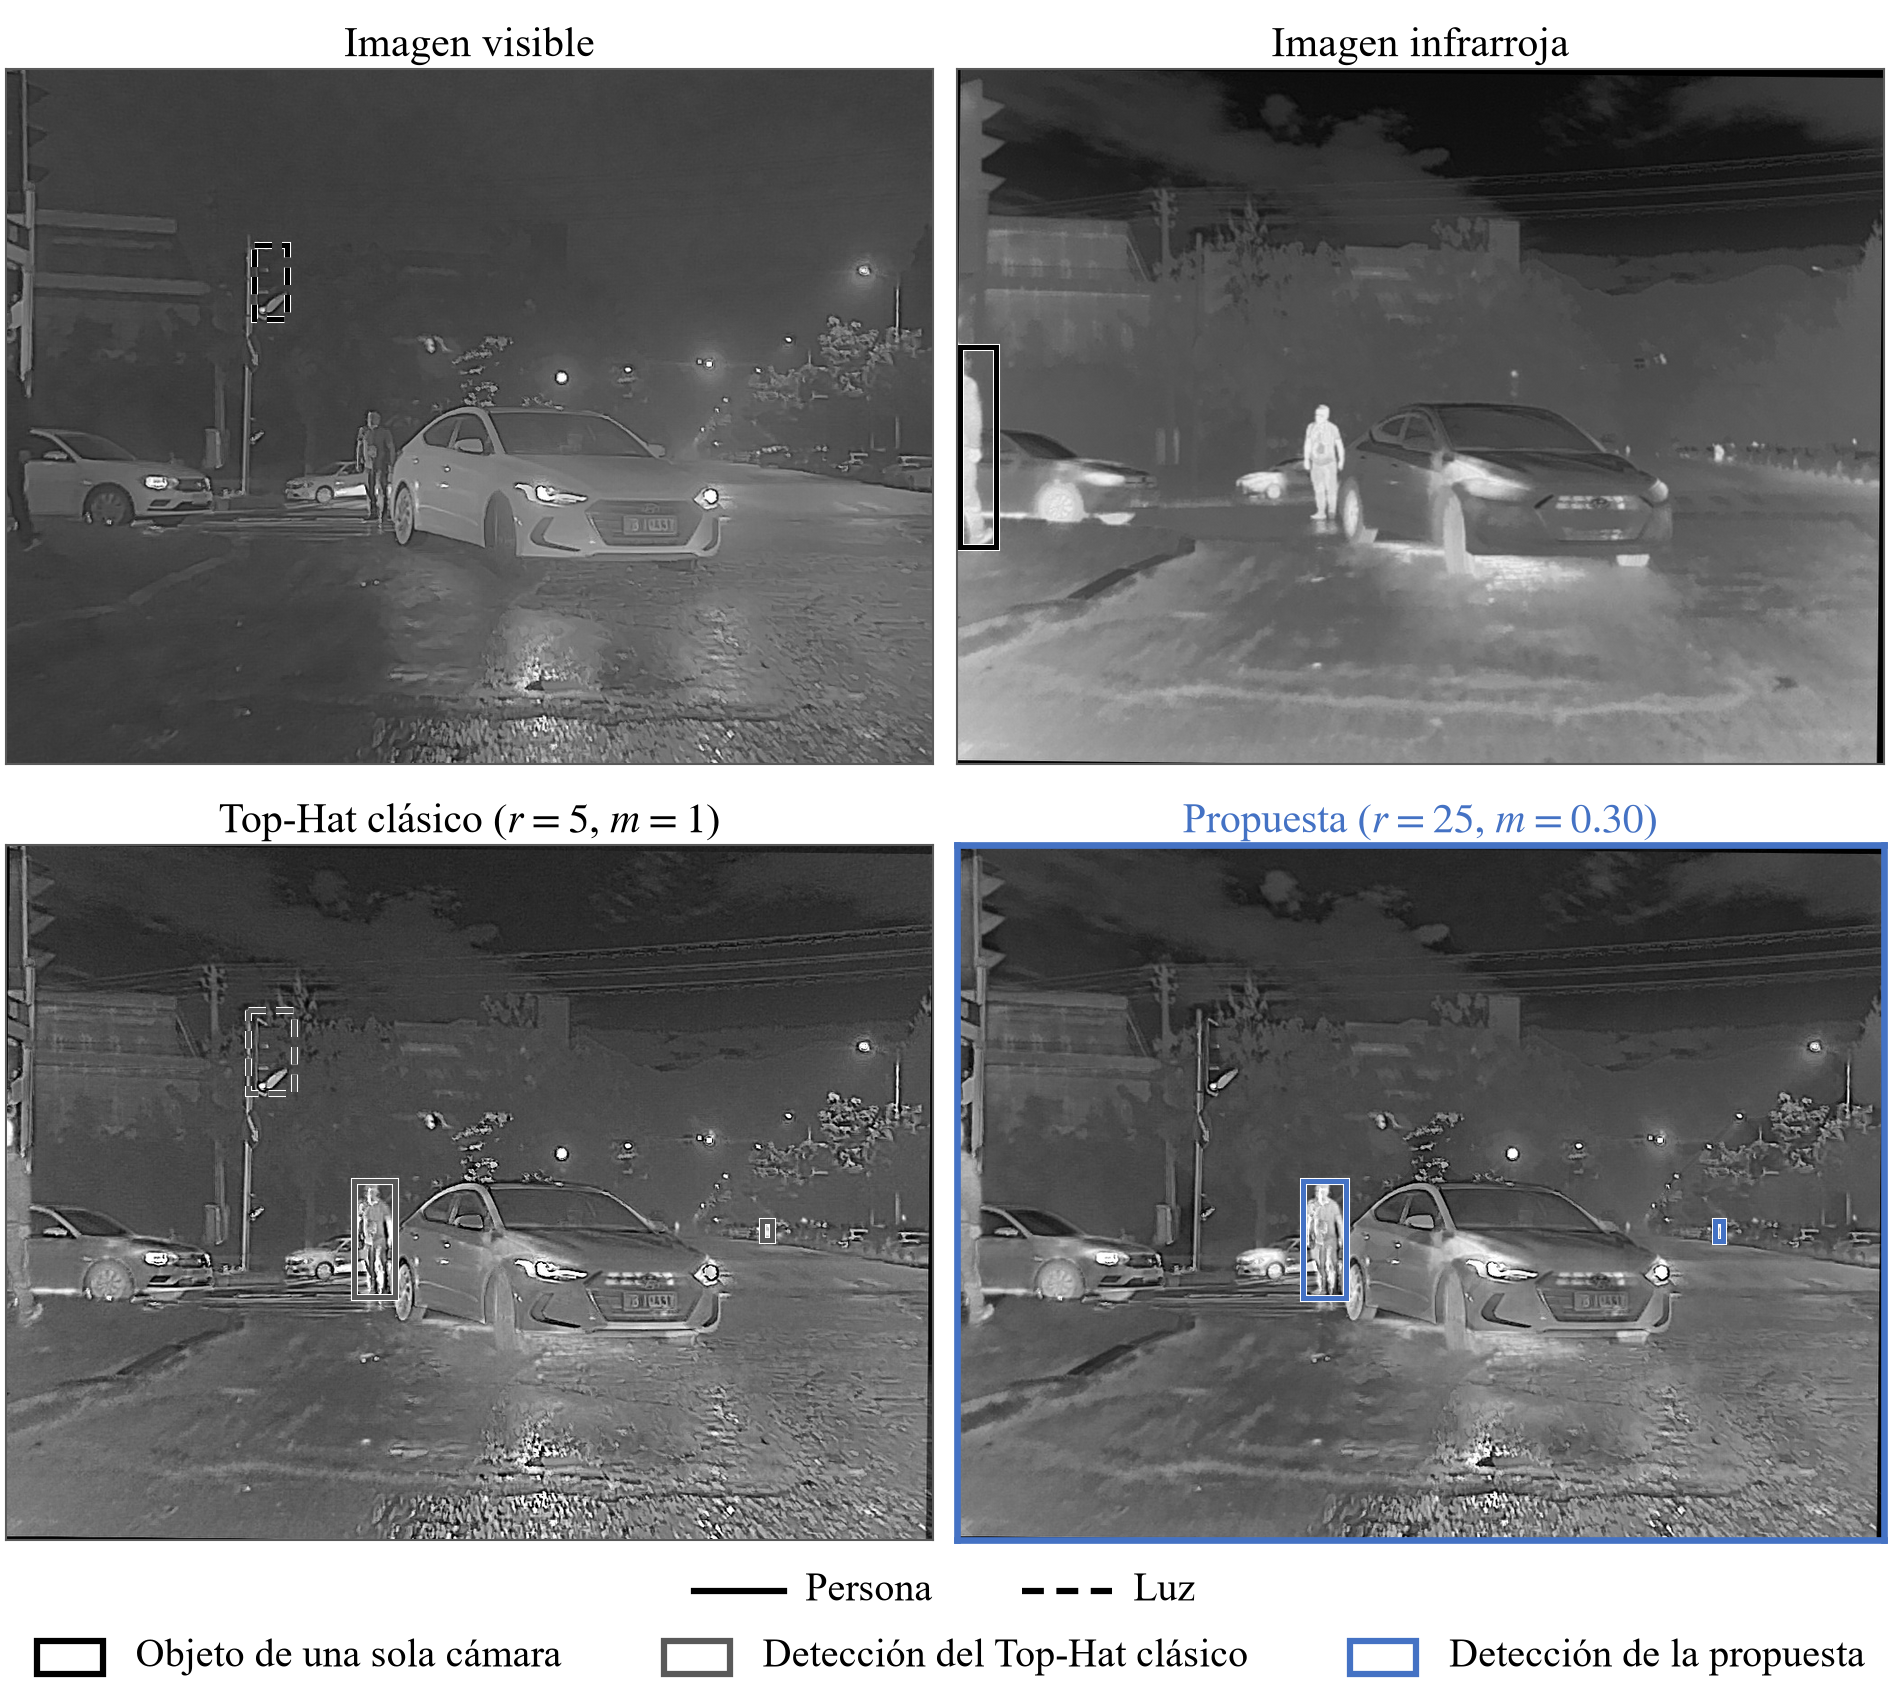
\includegraphics[width=\textwidth]{figuras/fig_m3fd_ejemplo}
\nota{Elaboración propia a partir de imágenes de M3FD \parencite{liu2022}. Es el cuadro 437 del
conjunto y pertenece a la prueba. Se eligió sin mirar las detecciones de las fusiones. De los 49
cuadros con al menos un objeto de solo la visible y uno de solo la infrarroja, 12 tienen marcadas en
M3FD las dos clases del análisis, personas y luces. Entre esos 12, es el que tiene los objetos de una sola cámara más grandes. Arriba están
las fuentes en escala de grises, tal como las recibe el detector. En cada una, el recuadro negro
marca su objeto de una sola cámara. Abajo, cada fusión lleva las detecciones de su detector, con la primera
semilla y su umbral principal: 0.26 en el Top-Hat clásico y 0.25 en la propuesta. La línea continua
marca personas, y la discontinua, luces.}
\end{figure}

La Tabla~\ref{tab:v2_tasas} presenta la tasa de acierto de las ocho entradas fusionadas. Están ordenadas
por tasa equilibrada, que promedia la tasa sobre los objetos de solo la visible y la tasa sobre los de
solo la infrarroja. La visible y la infrarroja no figuran en ella, porque sus detectores son los que
definen los objetos de una sola cámara.

\begin{table}[htbp]
\centering
\caption{Tasa de acierto de las entradas fusionadas en la detección de objetos}
\label{tab:v2_tasas}
\begin{tabular}{lcccc}
\toprule
\textbf{Entrada} & \textbf{Solo visible} & \textbf{Solo infrarroja} & \textbf{Equilibrada} & \textbf{De ambas} \\
\midrule
Pirámide de Laplace & 60.5 & 72.5 & \textbf{66.5} & 97.1 \\
DTCWT & 53.7 & 72.2 & 62.9 & 94.1 \\
DWT (Haar) & 53.7 & 70.9 & 62.3 & 95.9 \\
Propuesta & 55.6 & 67.2 & 61.4 & 94.4 \\
DWT (db4) & 51.2 & 69.2 & 60.2 & 96.0 \\
Promedio simple & 49.1 & 71.3 & 60.2 & 95.1 \\
Top-Hat clásico & 51.3 & 65.5 & 58.4 & 94.1 \\
Pirámide de razón & 49.0 & 57.3 & 53.1 & 93.0 \\
\bottomrule
\end{tabular}
\nota{Elaboración propia. Las tasas están en porcentaje y se calcularon con el umbral principal. El umbral principal de cada detector se fijó para que este cometiera, en los cuadros de seguimiento, tantos falsos positivos de personas y luces por imagen como los detectores de la visible con un umbral de 0.25. Solo visible y Solo infrarroja se calculan sobre los objetos que ve una sola cámara: 211 vistos solo por la visible y 622 solo por la infrarroja. La columna De ambas se calcula sobre los 724 objetos que ven las dos cámaras. La columna Equilibrada es el promedio de las dos columnas anteriores. Las filas van de mayor a menor tasa equilibrada, y la mayor está en negrita. Cada tasa promedia, sobre tres semillas, la fracción de objetos encontrados. La visible y la infrarroja no figuran porque sus detectores definen qué objetos ve una sola cámara. Propuesta: el algoritmo de fusión presentado en este trabajo.}
\end{table}


La pirámide de Laplace obtuvo la mayor tasa equilibrada, 66.5~\%. La propuesta quedó cuarta de ocho,
con 61.4~\%, y el Top-Hat clásico, séptimo, con 58.4~\%. El Top-Hat clásico quedó así por debajo del
promedio simple, que obtuvo 60.2~\%, aunque esa diferencia no se sometió a prueba.

Al separar las dos tasas que forman la equilibrada, la propuesta fue segunda en los objetos vistos solo
por la visible, con 55.6~\%, detrás de la pirámide de Laplace. En los vistos solo por la infrarroja fue
sexta, con 67.2~\%. Sobre los objetos que veían las dos cámaras, todas las entradas alcanzaron al menos
el 93.0~\%. Con el umbral fijo de 0.25, la propuesta obtuvo una tasa equilibrada de 61.1~\% y quedó
cuarta; con el de mejor equilibrio por clase, obtuvo 59.0~\% y quedó quinta.

La Figura~\ref{fig:m3fd_aciertos} muestra dos escenas de la prueba con un objeto de una sola cámara,
uno de cada cámara, que el detector de la propuesta encontró. Arriba, en un cuadro nocturno, la
persona de la derecha apenas se distingue del fondo en la imagen visible y se ve nítida en la
infrarroja. Con la primera semilla, el detector de la visible no la encontró, y sí los de la
infrarroja, del Top-Hat clásico y de la propuesta. Abajo, en un cuadro diurno, la imagen visible
muestra encendidas las flechas de los dos semáforos y el número del de la derecha; en la infrarroja,
los dos son manchas claras sin esos detalles. Con la primera semilla, los detectores de la visible, del
Top-Hat clásico y de la propuesta encontraron el semáforo de la derecha, y el de la infrarroja no. En
toda la prueba, las dos fusiones coincidieron en la mayoría de estos objetos: con esa misma semilla, de
los que encontró al menos una de ellas, las dos encontraron 83 de 143 de solo la visible y 355 de 460
de solo la infrarroja. Como la Figura~\ref{fig:m3fd_ejemplo}, esta
ilustra cómo una fusión puede encontrar un objeto que una de las cámaras pierde, y no el resultado de
conjunto, que es el de la Tabla~\ref{tab:v2_tasas}.

\begin{figure}[htbp]
\centering
\caption{Detecciones en dos cuadros de M3FD con un objeto de una sola cámara}
\label{fig:m3fd_aciertos}
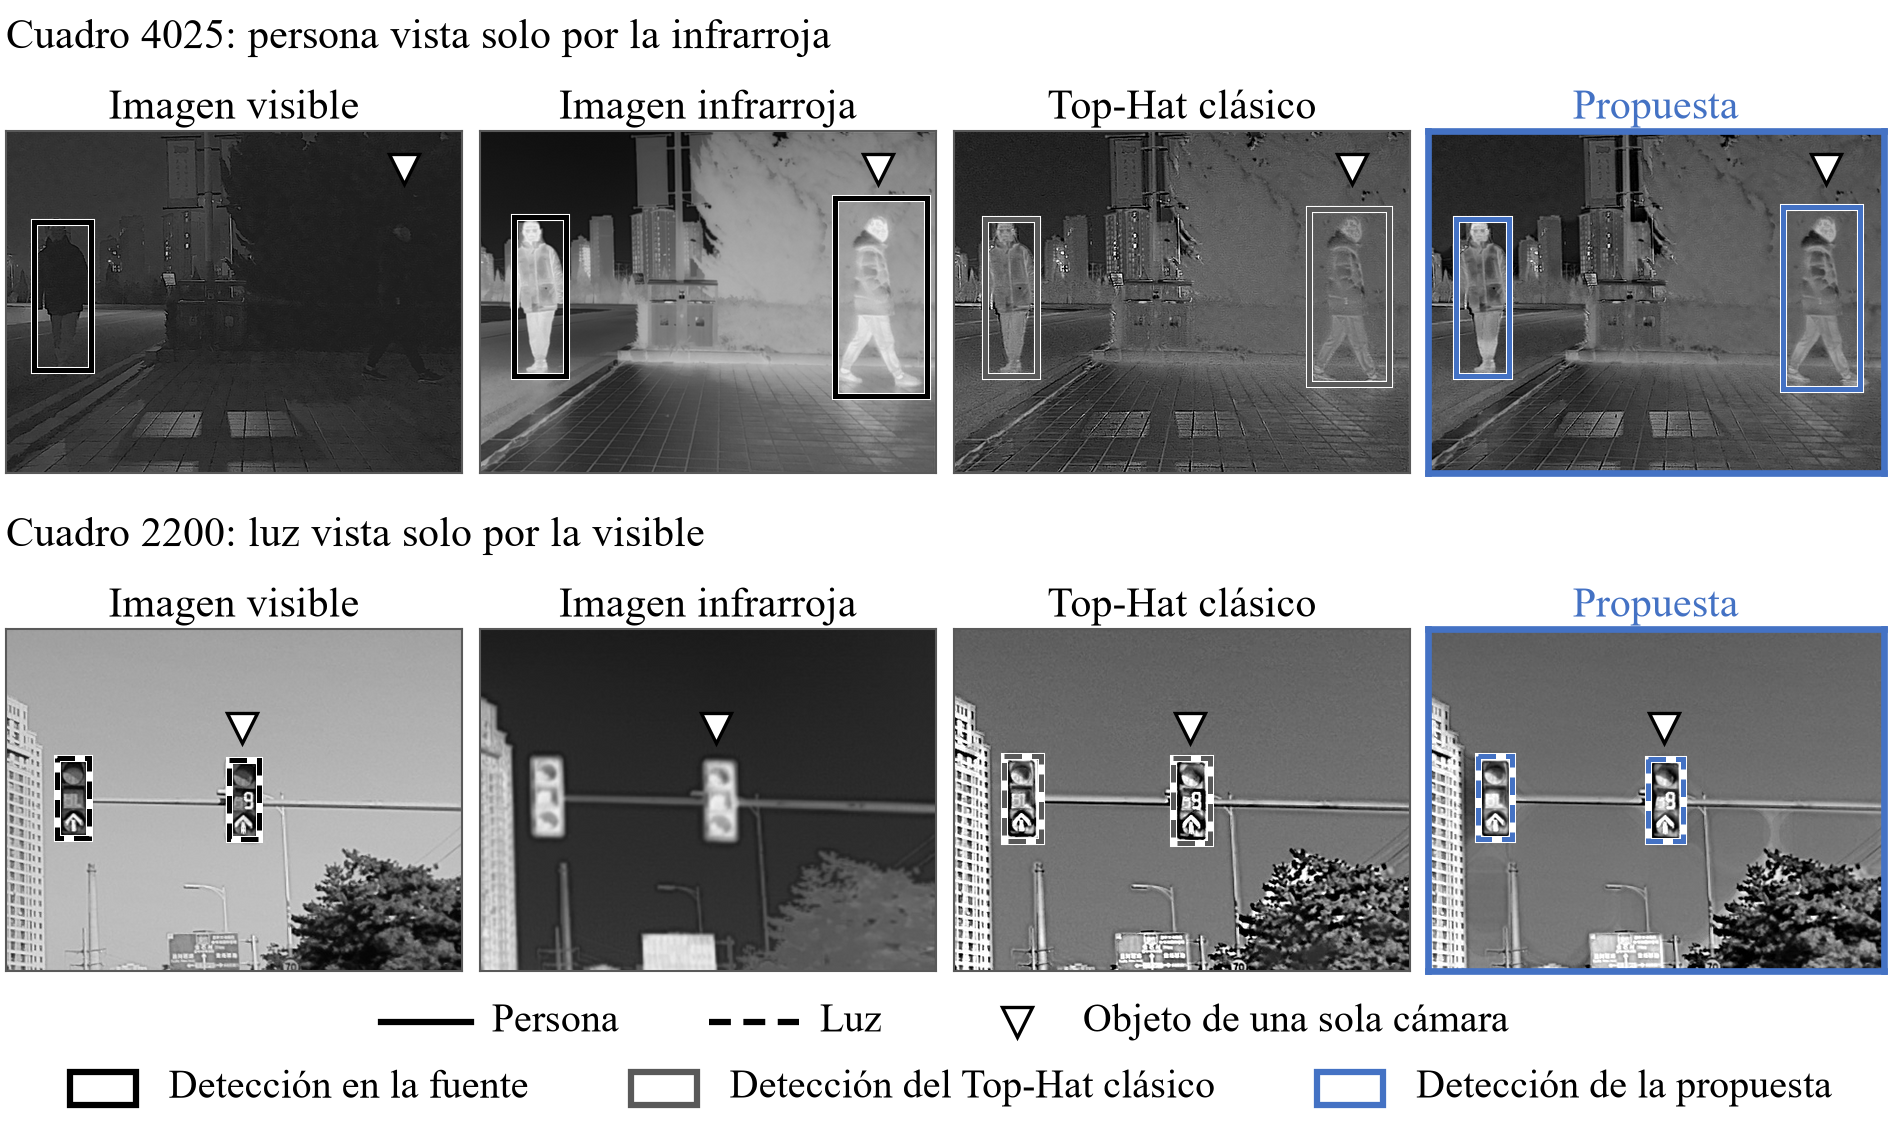
\includegraphics[width=\textwidth]{figuras/fig_m3fd_aciertos}
\nota{Elaboración propia a partir de imágenes de M3FD \parencite{liu2022}. Son los cuadros 4025 y 2200
del conjunto y pertenecen a la prueba. Se eligieron con una regla fija que no usa las detecciones del
Top-Hat clásico. Entre los objetos de una sola cámara que encontró el detector de la propuesta con la
primera semilla, fuera del grupo del cuadro 437 de la Figura~\ref{fig:m3fd_ejemplo}, arriba está el de
solo la infrarroja de mayor área según su marca en M3FD, y abajo, el de solo la visible de mayor área
entre los de otro grupo que el de arriba. Como la regla parte de los objetos que encontró la
propuesta, la figura no indica con qué frecuencia los encuentra. Arriba se muestra el cuadro entero,
y abajo, un recorte de $475 \times 356$ píxeles alrededor del objeto, el mismo en los cuatro paneles.
Cada panel lleva las detecciones de su detector con la primera semilla y el umbral principal: 0.25 en
la visible y en la propuesta, y 0.26 en la infrarroja y en el Top-Hat clásico. Los objetos de una sola
cámara se definen con los tres detectores de cada cámara, y los paneles muestran solo el primero. Por
eso, abajo, el de la infrarroja tampoco encuentra el semáforo de la izquierda, que es de las dos
cámaras porque lo encontraron los otros dos detectores de la infrarroja. El triángulo
señala el objeto de una sola cámara. A diferencia de la Figura~\ref{fig:m3fd_ejemplo}, los recuadros
negros no son objetos marcados, sino detecciones en las fuentes; los gris oscuro, del Top-Hat clásico
($r = 5$, $m = 1$), y los azules, de la propuesta ($r = 25$, $m = 0.30$). La línea continua marca
personas, y la discontinua, luces.}
\end{figure}

\subsection{Comparación con el Top-Hat clásico}
\label{sec:res-tophat}

La Tabla~\ref{tab:deteccion_tophat} reúne la diferencia de tasa equilibrada entre la propuesta y el
Top-Hat clásico, con su intervalo de confianza del 95~\%, para cada umbral y para el \textit{bootstrap}
salvaje por grupos.

\begin{table}[htbp]
\centering
\caption{Diferencia de tasa equilibrada entre la propuesta y el Top-Hat clásico}
\label{tab:deteccion_tophat}
\begin{tabular}{lcc}
\toprule
\textbf{Cálculo} & \textbf{Diferencia} & \textbf{Intervalo del 95~\%} \\
\midrule
Umbral principal & 3.0 & [0.0, 6.0] \\
Umbral fijo de 0.25 & 2.7 & [0.0, 5.3] \\
Umbral de mejor equilibrio por clase & 2.5 & [1.1, 3.9] \\
\addlinespace \textit{Bootstrap} salvaje por grupos & 3.0 & [$-$3.5, 5.5] \\
\bottomrule
\end{tabular}
\nota{Elaboración propia. La diferencia, en puntos porcentuales, es la tasa de acierto equilibrada de la propuesta menos la del Top-Hat clásico. El cálculo de los intervalos de confianza del 95~\% se describe en la Sección~\ref{sec:det-comparacion}. La unidad del análisis es el grupo de bloques contiguos de cuadros: de los once grupos de la prueba, entran los diez que tienen objetos de una sola cámara. Las tres primeras filas usan un error estándar robusto por grupos y la distribución $t$ con nueve grados de libertad \parencite{cameron2015}. La última fila usa el umbral principal y un \textit{bootstrap} salvaje por grupos, estudentizado y con la hipótesis nula impuesta \parencite{cameron2008, webb2023}. Su intervalo reúne las diferencias que esa prueba no rechaza al 5~\%, y el valor $p$ para una diferencia nula es 0.17. Los límites inferiores que se muestran como 0.0 son positivos: 0.02 puntos con el umbral principal y 0.05 con el umbral fijo. Según el par de semillas, la diferencia va de $-$3.1 a 7.8 puntos con el umbral principal. Con el umbral fijo va de $-$2.9 a 7.1, y con el de mejor equilibrio por clase, de $-$5.2 a 9.1. Con cada umbral, tres de las nueve diferencias son negativas: frente a una misma semilla del Top-Hat clásico, las tres semillas de la propuesta quedan por debajo. Por eso la diferencia no es robusta a la semilla.}
\end{table}


Con el umbral principal, la propuesta aventajó al Top-Hat clásico, pero el intervalo de confianza apenas
dejó fuera el cero. Su tasa equilibrada fue 3.0 puntos porcentuales mayor, con un intervalo de 0.0 a
6.0. El límite inferior exacto fue de 0.02 puntos, que con un decimal se muestra
como 0.0. La diferencia, además, no es robusta a la semilla: según el par de semillas, va de $-3.1$ a
7.8 puntos.

Con el umbral fijo de 0.25, la diferencia fue de 2.7 puntos, con un intervalo de 0.0 a 5.3 y un límite
inferior exacto de 0.05. Con el umbral de mejor equilibrio por clase fue de 2.5 puntos, con un intervalo
de 1.1 a 3.9. Los tres intervalos calculados con la distribución $t$ dejaron fuera el cero, los dos
primeros por muy poco. El \textit{bootstrap} salvaje por grupos, estudentizado y con la hipótesis nula
impuesta, no lo excluyó. Con el umbral principal dio un valor de $p$ de 0.17 y un intervalo de $-$3.5 a
5.5, y con los otros dos umbrales, valores de $p$ de 0.17 y 0.08. Al dejar fuera el grupo mayor de la
prueba, la diferencia con el umbral principal bajó de 3.0 a 1.5 puntos; al dejar fuera cualquiera de
los otros, quedó entre 2.3 y 3.6.

La Figura~\ref{fig:deteccion_tasas} muestra la tasa equilibrada de cada semilla en las ocho entradas
fusionadas y las nueve diferencias entre las semillas de la propuesta y las del Top-Hat clásico. Las
tres semillas de la propuesta quedaron a menos de un punto entre sí, mientras que las del Top-Hat
clásico se separaron casi diez. Por eso las diferencias entre pares de semillas no mantuvieron el signo.
Con el umbral principal, seis fueron positivas y tres negativas, de $-2.2$, $-3.1$ y $-2.3$ puntos. Las
tres negativas se dieron frente a la misma semilla del Top-Hat clásico, la de tasa más alta, que superó
a las tres de la propuesta. Con los otros dos umbrales hubo también tres diferencias negativas, otra vez
frente a esa semilla. Según el par de semillas, la diferencia fue de $-2.9$ a 7.1 puntos con el umbral
fijo de 0.25 y de $-5.2$ a 9.1 con el de mejor equilibrio por clase.

Como referencia, con el mismo cálculo, la diferencia entre la propuesta y el promedio simple fue de 1.2
puntos, con un intervalo de $-6.6$ a 9.0, que incluye valores de los dos signos. Frente a la pirámide de
Laplace, la propuesta quedó por debajo en los nueve pares de semillas, con diferencias de $-5.8$ a
$-4.6$ puntos.

\begin{figure}[htbp]
\centering
\caption{Tasa equilibrada por entrada y diferencia entre la propuesta y el Top-Hat clásico}
\label{fig:deteccion_tasas}
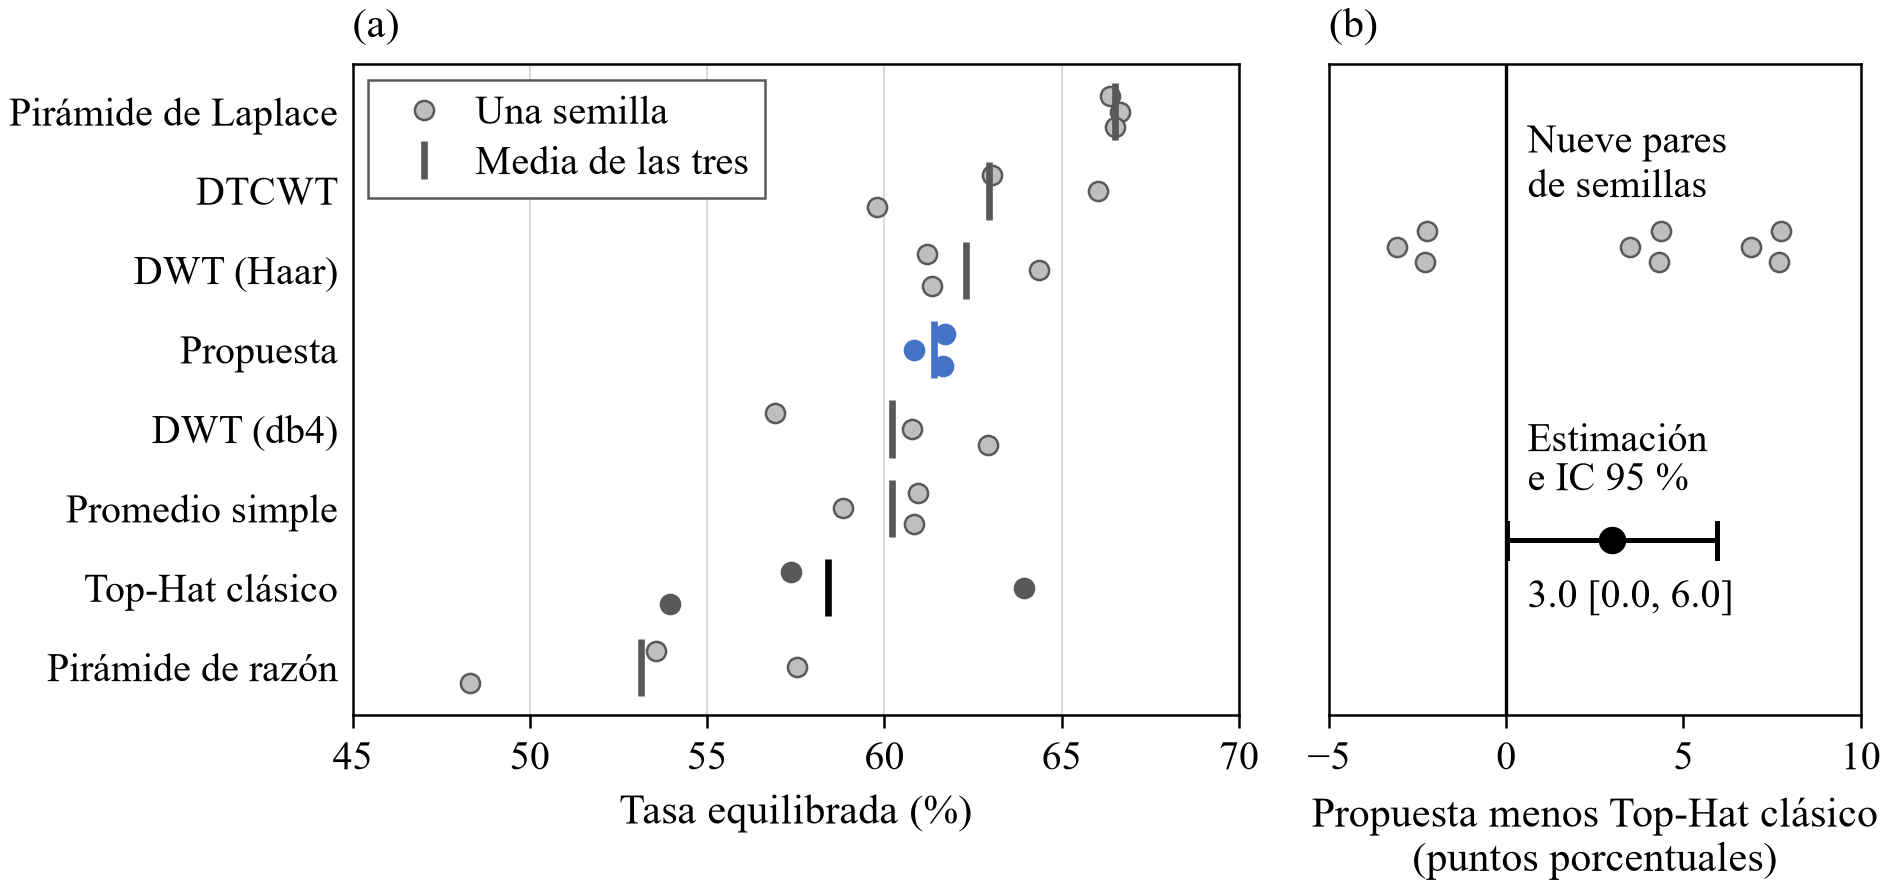
\includegraphics[width=\textwidth]{figuras/fig_deteccion_tasas}
\nota{Elaboración propia. Las tasas corresponden al umbral principal. (a) Las ocho entradas fusionadas
de la Tabla~\ref{tab:v2_tasas}, ordenadas de mayor a menor tasa. Cada punto es la tasa de una semilla del detector,
y la línea vertical, la media de las tres semillas, que es el valor de la tabla. La propuesta está en azul y el Top-Hat
clásico, en gris oscuro, con su media en negro. (b) Diferencia de tasa equilibrada, propuesta menos
Top-Hat clásico, en puntos porcentuales. Arriba están las nueve diferencias entre cada semilla de la propuesta y cada semilla del
Top-Hat clásico. Abajo están la estimación principal y su intervalo, con los límites entre corchetes. A
la derecha del cero, la propuesta acierta más que el Top-Hat clásico. Los dos paneles tienen la misma
escala horizontal: un punto porcentual mide lo mismo en ambos. IC 95~\%: intervalo de confianza del
95~\%.}
\end{figure}

La ventaja de la propuesta frente al Top-Hat clásico es, entonces, mínima y depende de la semilla, por
lo que queda como un hallazgo por confirmar.

\subsection{Medidas secundarias y entrenamiento}
\label{sec:res-secundarias}

La mAP50, la precisión media global sobre las seis clases, se midió en los 1197 cuadros que dejó el
primer filtro (Sección~\ref{sec:det-datos}). En esta medida, la propuesta quedó séptima de diez, por
debajo del Top-Hat clásico. La pirámide de Laplace obtuvo el mayor valor, 0.441, muy cerca de la DTCWT,
con 0.440, y del promedio simple, con 0.439. Siguieron el Top-Hat clásico, con 0.434, la DWT (db4), con
0.430, la infrarroja sola, con 0.429, y la propuesta, con 0.427. Cerraron la lista la DWT (Haar), con
0.415, la pirámide de razón, con 0.411, y la visible sola, con 0.363.

Así, cinco de las ocho entradas fusionadas superaron en mAP50 a la infrarroja sola. La propuesta no
estuvo entre ellas: quedó apenas por debajo, con 0.427 frente a 0.429, una diferencia menor que la
variación entre sus propias semillas, que fue de 0.419 a 0.440.

En los 49 cuadros con al menos un objeto de solo la visible y uno de solo la infrarroja, los detectores
de la propuesta encontraron al menos uno de cada tipo en el 57.1~\% de los casos. Con el Top-Hat
clásico la proporción fue algo mayor, 57.8~\%, y con la pirámide de Laplace llegó al 72.1~\%. Sobre los
objetos vistos por las dos cámaras, la propuesta y el Top-Hat clásico quedaron casi iguales, con 94.4~\% y 94.1~\%.
Ninguna de estas diferencias, ni las de mAP50, se sometió a prueba.

El seguimiento época por época se hizo solo con la primera semilla de cada entrada, midiendo la mAP50
sobre los 474 cuadros de seguimiento. Esos cuadros provienen de los mismos bloques que el
entrenamiento. En la época 40, su mAP50 fue de 0.73 a 0.76, muy superior a la de esos mismos detectores en los
1197 cuadros, de 0.35 a 0.46. Por eso, ese seguimiento refleja más el ajuste a cuadros parecidos a los de entrenamiento que la
capacidad de generalizar. Al final del entrenamiento, esa medida seguía subiendo en
casi todos los detectores: en las últimas cinco épocas, nueve de los diez tenían todavía una pendiente
positiva. La excepción fue el de la DWT (Haar). Entre las épocas 30 y 40 cambió, además, el orden de la propuesta
frente a dos métodos. En la época 30 quedaba por debajo de la pirámide de Laplace y de la DWT (db4), y
en la 40, por encima de ambas. En ese tramo, la propuesta pasó de 0.7347 a 0.7636; la pirámide de
Laplace, de 0.7406 a 0.7616, y la DWT (db4), de 0.7372 a 0.7512.

Por último, se calculó la correlación de Spearman entre el rango promedio de calidad, con 1 para el
mejor, y la tasa equilibrada de los siete métodos. Resultó de $\rho = -0.32$, con $p = 0.48$. El signo
negativo indica que los métodos mejor ubicados en calidad detectaron algo más, pero la correlación no
fue significativa. Los dos órdenes, además, provienen de conjuntos distintos: el de calidad, del TNO, y
el de detección, de M3FD.

\section{Examen de la hipótesis}
\label{sec:res-hipotesis}

Esta sección reúne, para cada afirmación de la hipótesis (Capítulo~\ref{cap:introduccion}), los
resultados con que se la examina según la Sección~\ref{sec:examen-hipotesis}. No se hizo ninguna prueba
nueva: todos los valores provienen de las secciones anteriores.

La primera afirmación compara la calidad de la propuesta con la del Top-Hat clásico. En los seis
contrastes de Wilcoxon con la corrección de Holm, la propuesta ganó en entropía, desviación estándar,
información mutua y similitud estructural (Tabla~\ref{tab:wilcoxon_resumen}). Perdió en gradiente medio
y empató en relación señal-ruido de pico, donde el $p$ corregido fue de 0.674. Como complemento, el rango
promedio fue de 3.642 en la propuesta, primera de siete, y de 4.242 en el Top-Hat clásico, sexto.

La segunda afirmación se refiere a los cinco métodos multiescala. Con las seis métricas, la propuesta
encabezó la clasificación por rango promedio: obtuvo 3.642, frente a 3.783 de la DTCWT. El margen, de
0.14 puestos, no tiene una prueba propia. Con las nueve métricas iniciales también quedó primera, y con
las diecisiete, tercera. Su perfil fue desigual entre los dos grupos de métricas. Ganó los cinco contrastes
de entropía y de gradiente medio, y cuatro de cinco en desviación estándar. Perdió los cinco de
similitud estructural y cuatro de cinco en información mutua y en relación señal-ruido de pico. Por
grupos de métricas, su rango promedio fue el mejor de los siete en actividad, 1.717, y el sexto en
fidelidad, 5.567.

La tercera afirmación corresponde a la aplicación. Con el umbral principal, la tasa equilibrada de la
propuesta superó a la del Top-Hat clásico en 3.0 puntos, con un intervalo de 0.0 a 6.0 y un límite
inferior exacto de 0.02. Esa diferencia no es robusta a la semilla: entre los nueve pares de semillas
fue de $-3.1$ a 7.8 puntos, y cada uno de los tres umbrales dejó tres diferencias negativas. Con los
otros dos umbrales, el límite inferior del intervalo también quedó por encima de cero. El
\textit{bootstrap} salvaje por grupos, en cambio, no excluyó el cero: con el umbral principal, su valor
de $p$ fue de 0.17.

Con esos resultados, la parte de la hipótesis que trata de la calidad se sostiene en lo principal. La
propuesta superó al Top-Hat clásico en cuatro de las seis métricas, y su calidad fue comparable a la de los cinco
métodos multiescala. Su primer puesto por rango promedio se apoya en un margen estrecho, sin una prueba
propia, y cambia con el conjunto de métricas. En la aplicación, la ventaja frente al Top-Hat clásico es
mínima: el límite inferior del intervalo apenas superó el cero, el \textit{bootstrap} no lo excluyó y
la diferencia no es robusta a la semilla. Esa parte de la hipótesis queda, por eso, como un hallazgo que falta confirmar con más grupos,
más semillas y otros detectores (Capítulo~\ref{cap:recomendaciones}).
